\label{chapter:quantum-convolution}\label{chap:quantum-convolution}
In the previous chapter we presented a quantum algorithm for exact string matching based on amplitude amplification used in Grover's quantum search algorithm. In this chapter we present a quantum algorithm for solving the approximate string matching problem using the concept of convolution of sequences. This algorithm makes use of the Fourier transform used in Shor's period finding algorithm. We present an intuition of the algorithm in Section~\ref{sec:qcon-prelims} and its application to the approximate string matching problem in Section~\ref{sec:application-to-approximate-string-matching}. We analyze the algorithms time and space complexity in Section~\ref{sec:time-space-complexity}. In Section~\ref{sec:sub-routines} we discuss in detail the sub-routines of the algorithm. Lastly, in Section~\ref{sec:quantum-algorithm-2} we define the algorithm.

\section{Preliminary concepts}\label{sec:qcon-prelims}
\subsection{Convolution of sequences}
The concept of \textit{convolution} is intuitively a process of applying some given transformation into an input of which the output describes some sense of correlation or similarity between the individual elements of the input and that of the transformation. Convolution has found application in areas such as linear time-invariant systems in which given an impulse function, an input impulse signal is transformed into an output signal that can be expressed as a linear combination of the transformed individual components of the input signal. Also, in image processing, it is used in identifying a location of a template within a much larger 2-dimensional image. In the resulting convolution of the template and the image, the location of the template in the image has the highest correlation value as compared to other locations in the image.

Convolution is defined on two input sequences of numerical values. An input signal and an impulse function can be expressed as a sequence of numerical values along the time domain while a a 2-dimensional image and a template can be expressed as 2-dimensional matrices of numerical values. We define the concept of convolution formally in Definition~\ref{def:convolution}

\begin{definition}[Convolution of sequence of real number]
	\label{def:convolution}
	The \textbf{convolution} of two sequences of real numbers $x=x_0,\ldots,x_{L-1}, y=y_0,\ldots,y_{L-1}$ is defined to be the sequence $z=z_0,\ldots,z_{L-1}$ given by
	\begin{equation}\label{eqn:convolution}
		z_{i} = \sum_{j=0}^{L-1} x_j \cdot y_{i-j}\ \ \text{for}\ i = 0, 1, \ldots, L-1
	\end{equation}
	where the operation between $x_j$ and $y_{i-j}$ is multiplication and the subscripts are taken (\textrm{mod} L).
\end{definition}
In this work, we use the usual notation $x \ast y$ for the convolution of any two arbitrary sequences $x, y$.

\subsection{Convolution as string matching}
The process of computing for the convolution of two sequences can be interpreted as the process of sliding a short sequence over a much longer sequence one position at a time. The \textit{i}-th value of the convolution of two sequences $x, y$ is given by
\begin{align*}
	z_{i} &= \sum_{j=0}^{L-1} x_j \cdot y_{i-j}\\
	        &= x_{0}\cdot y_{i} + x_{1}\cdot y_{i-1} + x_{2}\cdot y_{i-2} + \ldots + x_{L-1}\cdot y_{i-(L-1)}
\end{align*}
Let
\begin{itemize}
    \item $L=N+M-1$
    \item $x, y \in \{0,1\}^L$
    \item $x[N],\ldots,x[L-1]=0^{M-1}$
    \item $y[M],\ldots,y[L-1]=0^{N-1}$
\end{itemize}
Equation~\ref{eqn:convolution} then corresponds to the number of matching $1$s between the subsequences $x[i],\ldots,x[i+M-1]$ and $y[M-1],\ldots,y[0]$.

Let
\begin{itemize}
    \item $x_{\sigma_k}$ be given by
    	\begin{equation*}
			x[i]_{\sigma_k} =
			\begin{cases}
				1, & \mathrm{if}\ 0 \leq i < N\ \text{and T}[i]=\sigma_k\\
				0, & \mathrm{otherwise} 
			\end{cases}
		\end{equation*}
		for all $i=0,\ldots,L-1$
	\item $y_{\sigma_k}$ be given by
    	\begin{equation*}
			y[i]_{\sigma_k} =
			\begin{cases}
				1, & \mathrm{if}\ 0 \leq i < M\ \text{and P}[M-1-i]=\sigma_k\\
				0, & \mathrm{otherwise} 
			\end{cases}
		\end{equation*}
		for all $i=0,\ldots,L-1$
	\item $z_{\sigma_k} = x_{\sigma_k}*y_{\sigma_k}$
\end{itemize}
$z[i]_{\sigma_k}$ then corresponds to the number of matching presence of symbols $\sigma_k$ between subsequence $\mathrm{T}[i],\ldots,\mathrm{T}[i+M-1]$ and P.

Let
\begin{itemize}
    \item $\mathrm{T} \in \Sigma^{N}, \mathrm{P} \in \Sigma^{M}$ where $\Sigma=\{\sigma_1, \ldots, \sigma_k, \ldots\}$
    \item $x_{\sigma_k}=\mathrm{T}_{\sigma_k}0^{M-1}$ be the binary encoding of T with respect to symbol $\sigma_k$
    \item $y_{\sigma_k}=\mathrm{P}_{\sigma_k}[M-1],\ldots,\mathrm{P}_{\sigma_k}[0],0^{N-1}$ be the binary encoding of the reverse of P with respect to symbol $\sigma_k$
\end{itemize}
The point-wise addition of the convolutions $z_{\sigma_1}, \ldots, z_{\sigma_k}, \ldots$ then corresponds to a sequence $z_{\Sigma}$ given by
\begin{align}
	    z_{\Sigma}[i] &= \sum_{k=1}^{\vert \Sigma \vert} z_{\sigma_k}[i]\\
	                                          &= H\left( \mathrm{P}, \mathrm{T}[i],\ldots,\mathrm{T}[i+M-1] \right)\nonumber
\end{align}
for all $i=0,\ldots,L-1$. $z_{\Sigma}$ is a sequence of Hamming distance between P and each \textit{M}-length subsequence of T. Note that we are only interested with $z[M-1],\ldots,z[N-M+1]$ since 
\[
	z[M-1]=H\left(\mathrm{P}, \mathrm{T}[0],\ldots,\mathrm{T}[M-1]\right)
\]
and 
\[
	z[N-M+1]=H\left( \mathrm{P},\mathrm{T}[N-M+1],\ldots,\mathrm{T}[N-1]\right).
\]
The correspondence between the convolution of two sequences and the sequence of Hamming distance between subsequences of T and P implies that an efficient algorithm for computing the convolution is also an efficient algorithm for string matching. In the succeeding sections we present a quantum algorithm for computing the convolution of two sequences. This quantum algorithm, in specific cases, can be more efficient than its classical counterpart and other quantum algorithms for string matching presented in the previous chapter.

\subsection{Discrete Fourier transform and Convolution theorem}
%In signal processing and analysis, a theorem which describes the relationship between the convolution in the time domain and the frequency domain is the \textit{Convolution theorem}. In this work we use the convolution theorem specific to discrete periodic signals since the binary indicator sequences for the input text and pattern can be viewed as sampling of periodic signals but with noise. The transformation of an arbitrary signal from the time domain to the frequency domain is carried out using \textit{Fourier transform}. Since we are dealing only with discrete information, we are only interested in the \textit{discrete} version of the Fourier transform. 

One area of application of the concept of convolution is digital signal processing. There is a theorem which relates the convolution of two discrete signals in the time domain to operations on some transform of the discrete signals in the frequency domain. Such theorem is the \textit{Convolution theorem} in Theorem~\ref{thm:convolution-theorem}. The transform on the signals is the \textit{Fourier transform} and its inverse.

\begin{definition}[Discrete Fourier transform]
	Given a discrete signal $x=x_0,\ldots,x_{L-1}$, its discrete Fourier transform $X$ is given by
	\[
		X[k] = \frac{1}{\sqrt{L}} \sum_{l=0}^{L-1} x[j] e^{2\pi i k \frac{l}{L}}\ \text{for}\ k=0,\ldots,L-1
	\]
\end{definition}
\begin{definition}[Inverse discrete Fourier transform]
	Given a discrete signal $X$, for $l=0,\ldots,L-1$, its inverse discrete Fourier transform $x$ is given by
	\[
		x[k] = \frac{1}{\sqrt{L}} \sum_{l=0}^{L-1} X[j] e^{-2\pi i k \frac{l}{L}}\ \text{for}\ k=0,\ldots,L-1
	\]
\end{definition}
In this work we denote the discrete Fourier transform as \textit{F} and its inverse as $F^{-1}$.

\begin{theorem}[Convolution theorem]\label{thm:convolution-theorem}
	Given two discrete periodic signals $x=x_0,\ldots,x_{L-1}, y=y_0,\ldots,y_{L-1}$,
	\[
		F\left( x \ast y \right) = F\left( x \right) \cdot F\left( y \right)
	\]
where $\cdot$ denotes point-wise multiplication.
\end{theorem}

According to the Convolution theorem, the convolution in the time domain corresponds to point-wise multiplication in the frequency domain. The interest in the association of the concept of convolution with Fourier transform lies in the the availability of fast computation of the convolution of any two discrete periodic signals through efficient computation of the discrete Fourier transform. One algorithm which does efficient computation of the discrete Fourier transform is the \textit{fast Fourier transform algorithm}. Given an \textit{L}-length discrete signal $x$, its discrete Fourier transform will require $O(L^2)$ operations. The same computation can be achieved with $O(L\log_2(L))$ operations using the fast Fourier transform algorithm.

In this work, we compute for the discrete Fourier transform of a sequence using a quantum computer in the Convolution theorem. The following sections describe details of the quantum Fourier transform and the quantum version of the Convolution theorem. 

\subsection{Quantum Fourier transform}\label{subsec:qft}
The discrete Fourier transform of a sequence can be computed using a quantum computer. In Shor's quantum algorithm for prime factorization\cite{Shor1994}, he demonstrated a polynomial-time construction on a quantum computer for a unitary matrix which corresponds to the discrete Fourier transform. His construction on a quantum computer is for the special case when $L=2^n$, which was independently discovered and analyzed by Coppersmith in \cite{Coppersmith1994} and Barenco et. al in \cite{Barenco1996}. The quantum version of the discrete Fourier transform and its inverse is defined in Definition~\ref{def:qft} and Definition~\ref{def:iqft}.

\begin{definition}[Quantum Fourier transform]\label{def:qft}
	Let $B=\{\vert 0 \rangle, \ldots, \vert L-1 \rangle\}$ be an orthonormal basis for a $L$-dimension complex vector state space. The quantum Fourier transform is defined such that
	\[
		F_{\mathrm{Q}}\left(\vert k \rangle\right) = \frac{1}{\sqrt{L}} \sum_{j=0}^{L-1} e^{2\pi i k \frac{j}{L}} \vert j \rangle \ \ \ \text{ for all } \vert k \rangle \in B
	\]
\end{definition}

\begin{definition}[Inverse quantum Fourier transform]\label{def:iqft}
	Let $B=\{\vert 0 \rangle, \ldots, \vert L-1 \rangle\}$ be an orthonormal basis for a $L$-dimensional complex vector state space. The inverse quantum Fourier transform is defined such that
	\[
		F_{\mathrm{Q}}^{-1}\left(\vert k \rangle\right) = \frac{1}{\sqrt{L}} \sum_{j=0}^{L-1} e^{-2\pi i k \frac{j}{L}} \vert j \rangle \ \ \ \text{ for all } \vert k \rangle \in B
	\]
\end{definition}
The quantum Fourier transform can be implemented as the $L \times L$ unitary matrix given by
\[
	F_{\mathrm{Q}}(k,l) = \frac{1}{\sqrt{L}} e^{2\pi i k\frac{l}{L}}
\]
for all $k,l=0,\ldots,L-1$. Note that this is the same matrix as that of the discrete Fourier Transform. The inverse quantum Fourier transform on the other hand is given by 
\[
	F_{\mathrm{Q}}(k,l) = \frac{1}{\sqrt{L}} e^{-2\pi i k\frac{l}{L}}
\]
for all $k,l=0,\ldots,L-1$. On the other hand, the input sequence can be represented as a $1 \times L$ column vector $\left[ x_0, x_1, \ldots, x_{L-1} \right]^T$. The computation of the fast Fourier transform algorithm requires $O\left(L\log_2(L)\right)$ time complexity. The quantum Fourier transform though, as shown by Shor's quantum network construction, can be implemented using quantum circuit with depth of $O\left( \log_2(L)^2 + \log_2(L) \right)$, which is quadratic in the length of the input $\log_2(L)$. An approximation of the quantum Fourier transform has been shown to reduce the circuit complexity by a constant factor \cite{Coppersmith1994} by discarding some phase factors in the elements of the matrix. 

Since the matrix construction of the quantum Fourier transform is just same with that of the discrete Fourier transform, it seems that we can directly replace the discrete Fourier transform with the quantum Fourier transform in the Convolution theorem. This is not the case though as shown in \cite{Lomont2003}. There is no unitary operation which corresponds to point-wise multiplication of two Fourier transforms. A suggested unitary approximation of the point-wise multiplication in \cite{Curtis2004} is to construct an $L \times L$ matrix $V_{\mathrm{X}}$ of which entries $V_{\mathrm{X}}(i,i)$ correspond to the \textit{normalized entries} of the Fourier transform $\vert X \rangle$ of the input superposition quantum states $\vert x \rangle$ corresponding to input sequence $x[l]$. Note that $V_{\mathrm{X}}(i,i)$ is undefined when $\langle i \myket{X} = 0$. If such is the case, in this study we let $\langle i \myket{X} = \epsilon$ where $\epsilon$ is a very small real number. This implies $V_{\mathrm{X}}(i,i) = 1$ when $\langle i \myket{X} = 0$. We define formally this matrix in Definition~\ref{def:operator-V}.

\begin{definition}[Operator $V_\mathrm{X}$]\label{def:operator-V}
	Given the quantum Fourier transform of an L-dimension quantum state $\vert x \rangle$ spanned by basis set $B=\{\vert 0 \rangle,\ldots,\vert L-1 \rangle\}$,
	\[
		\vert X \rangle = \frac{1}{L} \sum_{j=0}^{L-1} \sum_{k=0}^{L-1} e^{2\pi i k \frac{j}{L} } \vert j \rangle,
	\]
	operator $V_{\mathrm{X}}$ is an $L \times L$ matrix given by
	\[
		V_{\mathrm{X}}(i,j) = 
		\begin{cases}
			\frac{\langle i \vert X \rangle}{\| \langle i \vert X \rangle \|}, & \mathrm{if\ } i=j,\mathrm{\ and\ } \langle i \myket{X} \neq 0,\\
			1,                                                                                       & \mathrm{if\ } i=j,\mathrm{\ and\ } \langle i \myket{X} = 0,\\
			0,                                                                                       & \mathrm{otherwise} 
		\end{cases}
	\]
	for all $i,j = 0,\ldots,L-1$.
\end{definition}

\begin{lemma}
	The operator $V_{\mathrm{X}}$ is a unitary. 
\end{lemma}
\begin{proof}
Since $V_{\mathrm{X}}$ is a diagonal matrix, $V_{\mathrm{X}}V_{\mathrm{X}}^\dagger $ is given by
\begin{equation*}
	\begin{split}
		\frac{\langle i \vert X \rangle}{\| \langle i \vert X \rangle \|}\frac{\langle i \vert X \rangle^\ast}{\| \langle i \vert X \rangle^\ast \|} &= \frac{\langle i \vert X \rangle}{ \sqrt{ \vert \langle i \vert X \rangle \vert^2} }\frac{\langle i \vert X \rangle^\ast}{ \sqrt{ \vert \langle i \vert X \rangle^\ast \vert^2 }}\\
		&= \frac{\langle i \vert X \rangle}{ \sqrt{ \langle i \vert X \rangle\langle i \vert X \rangle^\ast } }\frac{\langle i \vert X \rangle^\ast}{ \sqrt{ \langle i \vert X \rangle^\ast\langle i \vert X \rangle }}\\
		&= \frac{\langle i \vert X \rangle\langle i \vert X \rangle^\ast}{ \left(\sqrt{ \langle i \vert X \rangle\langle i \vert X \rangle^\ast } \right)^2 }\\
		&= \frac{\langle i \vert X \rangle}{ \langle i \vert X \rangle }\frac{\langle i \vert X \rangle^\ast}{ \langle i \vert X \rangle^\ast }\\
		&= 1
	\end{split}
\end{equation*}
for all $i=0,\ldots,L-1$. Thus, $V_{\mathrm{X}}V_{\mathrm{X}}^{\dagger}=I$. It is also easy to see to that $V_{\mathrm{X}}^{\dagger}V_{\mathrm{X}}=I$.
\end{proof}
Using the same analysis we used for the amplitude amplification operator $W$ in the previous chapter, we analyze the circuit and time complexity of operator $V_{\mathrm{X}}$. Since the elements along the diagonal of $V_{\mathrm{X}}$ will be less likely regular as composed to those along the diagonal of $W$, the phase context decomposition of operator $V_{\mathrm{X}}$ will require more than one single-parameter operators $V\left( \phi_i, l_i \right)$. Let \textit{q} be the number of distinct phase values $\phi_i$ along the diagonal of $V_{\mathrm{X}}$. The circuit complexity of approximating $V_{\mathrm{X}}$ using the Clifford+\textit{T} gate set will then be 
\[
	(q-1)C_0\log_2 \left( \frac{1}{\epsilon} \right) + \Om\left( \log\log \left(\frac{1}{\epsilon}\right) + (q-1)\log_2 L \right)
\]
\cite{Bocharov2015}. Assuming a low count of distinct phase values \textit{q} compared to \textit{L}, the circuit complexity of $V_{\mathrm{X}}$ will be in 
\[
	\Om\left( q\log_2 L \right).
\]
We assume the same for its time complexity. $V_{\mathrm{X}}$ will work on the same binary indicator sequence registers from the previous steps and so will work on $\log_2 L$ qubits.

Given the definition of operator $V_{\mathrm{X}}$, we define an approximate quantum version of the convolution theorem in Theorem~\ref{thm:quantum-convolution-theorem}.

\begin{theorem}[Quantum convolution theorem]\label{thm:quantum-convolution-theorem}
	Let $x$ and $y$ be two sequences of length L and $z = x \ast y$. Let $\vert x \rangle, \vert y \rangle, \vert z \rangle$ be quantum state representations of $x, y$ and $z$ spanned by basis set $B=\{\vert 0 \rangle,\ldots,\vert L-1 \rangle\}$, respectively. Given the quantum Fourier transform $\vert Y \rangle$ of $\vert y \rangle$ and the unitary operator $V_{\mathrm{X}}$ constructed from the quantum Fourier transform $\vert X \rangle$ of $\vert x \rangle$,
	\[
		F_{\mathrm{Q}}\left( \vert z \rangle \right) \approx V_{\mathrm{X}} \left(\vert Y \rangle\right)
	\]
where $V_{\mathrm{X}} \left(\vert Y \rangle\right)$ is given by
	\begin{equation*}
		\begin{split}
			\langle i \vert \left(V_{\mathrm{X}} \left(\vert Y \rangle\right)\right) &= \frac{\langle i \vert X \rangle}{\| \langle i \vert X \rangle \|} \langle i \vert Y \rangle
		\end{split}
	\end{equation*}
for all $i=0,\ldots,L-1$.
\end{theorem}
From Theorem~\ref{thm:quantum-convolution-theorem} we can derive an \textit{approximation} of $\vert z \rangle$ by taking the inverse quantum Fourier transform of $V_{\mathrm{X}} \left(\vert Y \rangle\right)$, 
\[
	\vert z \rangle \approx F_{\mathrm{Q}}^{-1}\left( V_{\mathrm{X}}\left( \vert Y \rangle \right) \right).
\]
Since an approximation of \textit{z} is encoded in the quantum state, $F_{\mathrm{Q}}^{-1}\left( V_{\mathrm{X}}\left( \vert Y \rangle \right) \right)$, we can only get one classical output for each measurement of the state of the quantum register. We iterate the quantum convolution algorithm multiple times to obtain multiple classical values corresponding to indices in T. These indices will be interpreted as possible solution starting indices of exact or approximate copies of P in T. Just like in classical convolution, we will only consider the middle $N-M+1$ indices of the convolution as valid candidate solutions. Basic classical verification of an output will only require time complexity linear to the size of the input pattern $M$.

\section{In application to approximate string matching}\label{sec:application-to-approximate-string-matching}
%In \cite{Fischer1974} the concept of convolution was shown to be also applicable to the string matching problem. Given input text T and pattern P, we encode the sequences
%\begin{equation*}
%	\begin{split}
%		\text{T}_{\mathrm{pad}} &= \text{T}[0], \text{T}[1], \ldots, \text{T}[N-1], \ast^{M-1}\\
%		\text{P}_{\mathrm{pad}} &= \text{P}[M-1], \text{P}[M-2], \ldots, \text{P}[0], \ast^{N-1}.
%	\end{split}
%\end{equation*}
%Since we have sequences of symbols to compare, we replace the multiplication operation in the definition of convolution of two sequences of real numbers with a comparison operation. Let $L=N+M-1$. We define the convolution of two sequences of symbols in Definition~\ref{def:convolution-symbols}.
%
%\begin{definition}[Convolution of sequences of symbols]
%	\label{def:convolution-symbols}
%	The \textbf{convolution} of two sequences of symbols $x=\left(x_0,\ldots,x_{L-1}\right)$ and $y=\left(y_0,\ldots,y_{L-1}\right)$ defined over $\Sigma=\{\sigma_0,\ldots,\sigma_{\vert \Sigma \vert-1}\}$ is defined to be the sequence $z=\left(z_0,\ldots,z_{L-1}\right)$ given by
%	\[
%		z_{i} = \sum_{j=0}^{L-1} C(x_j, y_{i-j})\ \ \text{for}\ i = 0, 1, \ldots, L-1
%	\]
%	where C 
%	\[
%		C(x_j, y_{i-j}) =
%		\begin{cases}
%			0,\ \ \mathrm{if}\ x_j \neq y_{i-j}\ \mathrm{OR}\ (x_j = \ast\ \mathrm{OR}\ y_{i-j} = \ast), \\
%			1,\ \ \mathrm{otherwise}.
%		\end{cases}
%	\]
%	and the subscripts are taken (\text{mod} L).
%\end{definition}
%In Definition~\ref{def:convolution-symbols}, we let $x=\text{T}_{\mathrm{pad}}, y=\text{P}_{\mathrm{pad}}$ and \textit{z} the convolution of $\text{T}_{\mathrm{pad}}$ and $\text{P}_{\mathrm{pad}}$. The convolution of $\text{T}_{\mathrm{pad}}$ and $\text{P}_{\mathrm{pad}}$ will be the sequence of match scores for each \textit{M}-length substring of T compared with P, excluding the first and last $M-1$ indices in the convolution. The convolution of $\text{T}_{\mathrm{pad}}$ and $\text{P}_{\mathrm{pad}}$ then provides a solution to the approximate string matching problem if we select the indices \textit{i} in the z such that $M-z_i \leq d$ where \textit{d} is the input distance threshold.
%
%\begin{example}
%	Given input text \textrm{T} = a,a,b,a and pattern \textrm{P} = b,a, we identify the convolution of the sequences 
%		\begin{equation*}
%			\begin{split}
%				\textrm{T}_{\mathrm{pad}} = a,a,b,a,\ast\\
%				\text{P}_{\mathrm{pad}} = a,b,\ast,\ast,\ast
%			\end{split}
%		\end{equation*}
%	where $L = 5$. The convolution of $\text{T}_{\mathrm{pad}}$ and $\text{P}_{\mathrm{pad}}$ is given by
%		\begin{equation*}
%			\begin{split}
%				\gamma_0 &= \sum_{j=0}^{4} C(\text{T}_{\mathrm{pad}}[j],\overleftarrow{\text{P}}_{\mathrm{pad}}[0-j])\\
%				&= C(\text{T}_{\mathrm{pad}}[0],\overleftarrow{\text{P}}_{\mathrm{pad}}[0-0]) + C(\text{T}_{\mathrm{pad}}[1],\overleftarrow{\text{P}}_{\mathrm{pad}}[0-1]) + C(\text{T}_{\mathrm{pad}}[2],\overleftarrow{\text{P}}_{\mathrm{pad}}[0-2])\\
%				&\quad\quad\quad + C(\text{T}_{\mathrm{pad}}[3],\overleftarrow{\text{P}}_{\mathrm{pad}}[0-3]) + C(\text{T}_{\mathrm{pad}}[4],\overleftarrow{\text{P}}_{\mathrm{pad}}[0-4])\\
%				&= C(\text{T}_{\mathrm{pad}}[0],\overleftarrow{\text{P}}_{\mathrm{pad}}[0]) + C(\text{T}_{\mathrm{pad}}[1],\overleftarrow{\text{P}}_{\mathrm{pad}}[4]) + C(\text{T}_{\mathrm{pad}}[2],\overleftarrow{\text{P}}_{\mathrm{pad}}[3])\\
%				&\quad\quad\quad + C(\text{T}_{\mathrm{pad}}[3],\overleftarrow{\text{P}}_{\mathrm{pad}}[2]) + C(\text{T}_{\mathrm{pad}}[4],\overleftarrow{\text{P}}_{\mathrm{pad}}[1])\\
%				&= C(\text{T}_{\mathrm{pad}}[0],\text{P}[1]) + C(\text{T}_{\mathrm{pad}}[1],\ast) + C(\text{T}_{\mathrm{pad}}[2],\ast) + C(\text{T}_{\mathrm{pad}}[3],\ast) + C(\text{T}_{\mathrm{pad}}[4],\text{P}[0])\\
%				&= C\left(a,a \right) + C\left(a,\ast \right) + C\left(b,\ast \right) + C\left(a,\ast \right) + C\left(\ast,b \right)\\
%				&=1 + 0 + 0 + 0 + 0\\
%				&=1
%			\end{split}
%		\end{equation*}
%Following the same computation for $\gamma_1$ to $\gamma_4$, we will have the values $\gamma_1=1, \gamma_2=0, \gamma_3=2, \gamma_4=0$. The convolution of $\text{T}_{\mathrm{pad}}$ and $\overleftarrow{\text{P}}_{\mathrm{pad}}$ is then the sequence 1,1,0,2,0. Excluding the first and last 1 index of the convolution, the index with highest score in the convolution is index 3 which corresponds to index 2 of T. Index 2 of the convolution has score of 2 which corresponds to the number of matches when substring T[2,3] is compared to P.
%\end{example}
%
%\subsection{Binary indicator sequence encoding}
%Since we store data using binary quantum registers, we perform the comparison operation in Definition~\ref{def:convolution-symbols} as a binary operation on binary encoding of T and P. We use a \textit{binary indicator sequence} to encode an input sequence of symbols according to the presence or absence of a specific symbol in the sequence. A bit 1 will indicate the presence of a symbol and a bit 0 for , i.e. including the zero paddings to the right. Given an alphabet $\Sigma=\{\sigma_0,\ldots,\sigma_{\vert \Sigma \vert}\}$ on which the input text and pattern are defined, a binary indicator sequence will be created for each symbol $\sigma_i \in \Sigma$ for each of the text and pattern. We replace the compare operation $C(\cdot,\cdot)$ with the logical operation AND ($\wedge$). We redefine the convolution of two sequences of symbols in Definition~\ref{def:convolution-binary}.
%
%\begin{definition}[Convolution of binary sequences]
%	\label{def:convolution-binary}
%	The \textbf{convolution} of two binary sequences $S_1=\left(\alpha_0,\ldots,\alpha_{N-1}\right)$ and $S_2=\left(\beta_0,\ldots,\beta_{N-1}\right)$ is defined to be the sequence $S_3=\left(\gamma_0,\ldots,\gamma_{N-1}\right)$ given by
%	\[
%		\gamma_{i} = \sum_{j=0}^{N-1} \alpha_j \wedge \beta_{i-j}\ \ \text{for}\ i = 0, 1, \ldots, N-1
%	\]
%	where $\wedge$ is the logical AND operation and the subscripts are taken \text{(mod N)}.
%\end{definition}
%
%\begin{example}
%	Given $\Sigma=\{a,b\}$ and input text \text{T} = a,a,b,a and pattern \text{P} = b,a, we identify the convolution of the pairs of sequences for symbol \textit{a} as
%		\begin{equation*}
%			\begin{split}
%				\text{T}(a)_{\mathrm{pad}} = 1,1,0,1,0\\
%				\overleftarrow{\text{P}}(a)_{\mathrm{pad}} = 1,0,0,0,0
%			\end{split}
%		\end{equation*}
%	and symbol \textit{b} as
%		\begin{equation*}
%			\begin{split}
%				\text{T}(b)_{\mathrm{pad}} = 0,0,1,0,0\\
%				\overleftarrow{\text{P}}(b)_{\mathrm{pad}} = 0,1,0,0,0
%			\end{split}
%		\end{equation*}
%	We compute for the convolution of each pair of binary indicator sequences. The convolution of binary indicator sequences $\text{T}(a)_{\mathrm{pad}}$ and $\overleftarrow{\text{P}}(a)_{\mathrm{pad}}$ is given by
%	\begin{equation*}
%		\begin{split}
%			\gamma_{a_0} &= \sum_{j=0}^{4} \text{T}(a)_{\mathrm{pad}}[j] \wedge \overleftarrow{\text{P}}(b)_{\mathrm{pad}}[0-j]\\
%			&= \text{T}(a)_{\mathrm{pad}}[0] \wedge \overleftarrow{\text{P}}(b)_{\mathrm{pad}}[0-0] + \text{T}(a)_{\mathrm{pad}}[1] \wedge \overleftarrow{\text{P}}(b)_{\mathrm{pad}}[0-1] + \text{T}(a)_{\mathrm{pad}}[2] \wedge \overleftarrow{\text{P}}(b)_{\mathrm{pad}}[0-2]\\
%			&\quad\quad\quad\quad + \text{T}(a)_{\mathrm{pad}}[3] \wedge \overleftarrow{\text{P}}(b)_{\mathrm{pad}}[0-3] + \text{T}(a)_{\mathrm{pad}}[4] \wedge \overleftarrow{\text{P}}(b)_{\mathrm{pad}}[0-4]\\
%			&= \text{T}(a)_{\mathrm{pad}}[0] \wedge \overleftarrow{\text{P}}(b)_{\mathrm{pad}}[0] + \text{T}(a)_{\mathrm{pad}}[1] \wedge \overleftarrow{\text{P}}(b)_{\mathrm{pad}}[4] + \text{T}(a)_{\mathrm{pad}}[2] \wedge \overleftarrow{\text{P}}(b)_{\mathrm{pad}}[3]\\
%			&\quad\quad\quad\quad + \text{T}(a)_{\mathrm{pad}}[3] \wedge \overleftarrow{\text{P}}(b)_{\mathrm{pad}}[2] + \text{T}(a)_{\mathrm{pad}}[4] \wedge \overleftarrow{\text{P}}(b)_{\mathrm{pad}}[1]\\
%			&= 1 \wedge 1 + 1 \wedge 0 + 0 \wedge 0 + 1 \wedge 0 + 0 \wedge 0\\
%			&= 1 + 0 + 0 + 0 + 0\\
%			&= 1
%		\end{split}		
%	\end{equation*}
%	Following the same computation for the other scores, we get the values $\gamma_{a_1}=1, \gamma_{a_2}=0, \gamma_{a_3}=1, \gamma_{a_1}=0$. The convolution of the binary indicator sequences $\text{T}(a)_{\mathrm{pad}}$ and $\overleftarrow{\text{P}}(a)_{\mathrm{pad}}$ is then the sequence  1,1,0,1,0. Computing for the convolution of the binary indicator sequences $\text{T}(b)_{\mathrm{pad}}$ and $\overleftarrow{\text{P}}(b)_{\mathrm{pad}}$ on the other hand will arrive at the sequence 0,0,0,1,0. Adding the corresponding values of the two convolutions for symbols \textit{a} and \textit{b}, we get the sequence 1,1,0,2,0 which is also the sequence we got from computing the convolution of the sequence of symbols $\text{T}_{\mathrm{pad}}$ and $\overleftarrow{\text{P}}_{\mathrm{pad}}$.
%\end{example}

In this section we present an overview of how we apply the quantum convolution theorem into the problem of approximate string matching. Let $\text{T} \in \Sigma^N$ and $\text{P} \in \Sigma^M$ be input text and pattern sequences. Let $f_{\sigma}:\Sigma \rightarrow \{0,1\}$ be a function given by
\[
	f_{\sigma}(x)=
	\begin{cases}
		1, & x = \sigma,\\
		0, & \mathrm{otherwise.}
	\end{cases}
\]
We encode T and P into binary indicator sequences 
\begin{equation*}
	\begin{split}
		\text{T}_{\sigma}= f_{\sigma}\left(\text{T}[0]\right), \ldots, f_{\sigma}\left(\text{T}[N-1]\right),\ast^{M-1}\\
		\text{P}_{\sigma}= f_{\sigma}\left(\text{P}[M-1]\right), \ldots, f_{\sigma}\left(\text{P}[0]\right),\ast^{N-1}
	\end{split}	
\end{equation*}
for all $\sigma \in \Sigma$ and $\vert \{ i\ \text{where P}[i]=\sigma \} \vert > 0$. We then input each pair $\text{T}_{\sigma}, \text{P}_{\sigma}$ into the quantum convolution algorithm to arrive at a quantum superposition state $\vert z_{\sigma} \rangle$. Let $g:\Sigma \rightarrow \{0,\ldots,M-1\}$ be a function given by
\[
	g(\sigma)= i 
\]
such that $\text{P}[i]=\sigma$ and $\text{P}[j] \neq \sigma$ for all $j < i$. Function $g(\cdot)$ gives us the index of first occurrence of a symbol $\sigma$ in P. We measure the state of the quantum register in state $\vert z_{\sigma} \rangle$ to get a classical value $z_{\sigma}$ corresponding to an index in T. If the result of our measurement of the state of a quantum register in state $\vert z_{\sigma} \rangle$ during \textit{j}-th iteration of the quantum convolution algorithm is the classical value $z_{\sigma}^j$, then $z_{\sigma}^j - g(\sigma)$ corresponds to a possible starting location of an exact or approximate copy of P in T. Note that our measurement of the state of the quantum register in superposition state $\vert z_{\sigma_i} \rangle$ has no effect on the result of our measurement of the state of the other quantum registers in superposition state $\vert z_{\sigma_{l\neq i}} \rangle$. We thus can interpret the result of our measurement on each of the quantum registers independent of each other. Let $A_{\text{T},\text{P}}$, Table~\ref{tab:A_matrix}, be a matrix of the result of the measurement for each symbol $\sigma$ for each iteration $j=\{1,\ldots,K\}$ of the quantum convolution algorithm. Let the columns of this matrix be labeled $0,\ldots,K$ and its rows, $\sigma_1,\ldots,\sigma_m$, $m \leq M$. Let $A_{\text{T},\text{P}}$ be given by 
\[
	A_{\text{T},\text{P}}(i,j) = z_{\sigma_i}^j - g(\sigma_i)
\]
where $z_{\sigma_i}^j$ is the classical result of measurement of the quantum register in state $\vert z_{\sigma_i} \rangle$ for iteration \textit{j}, for all $i=1,\ldots,m$.

	\begin{table}[h!]
		\centering
		\begin{tabular}{| r || c | c | c | c | c |}
			\hline
			                   & 1 & 2 & 3 & \ldots & K\\
			\hline\hline
			$\sigma_1$ &    &    &    & \ldots &   \\ 
			\hline
			$\sigma_2$ &    &    &    & \ldots &   \\ 
			\hline
			\ldots          &    &    &    & \ldots &   \\ 
			\hline
			$\sigma_m$ &    &    &    & \ldots &   \\
			\hline
		\end{tabular}
		\caption{Matrix $A_{\text{T},\text{P}}$.}
		\label{tab:A_matrix}
	\end{table}
Let \textit{k} be our target number of solution starting indices to the approximate string matching problem given T and P. Let \textit{K} be our upper bound on the number of iterations for the quantum convolution algorithm. We iterate the quantum convolution algorithm for \textit{k} times, filling up matrix $A_{\mathrm{T},\mathrm{P}}$ during each iteration. Let $B_{\mathrm{T},\mathrm{P}}$ denote an ordered set of the unique values $A_{\text{T},\text{P}}(i,j)$ ordered according number of occurrence in $A_{\mathrm{T},\mathrm{P}}$. We classically verify if 
\[
	H\left(\text{P},\text{T}[B_{\mathrm{T},\mathrm{P}}(i)],\ldots,\text{T}[B_{\mathrm{T},\mathrm{P}}(i) + M - 1]\right) \leq d
\] 
for all $i=0,\ldots,\vert B_{\mathrm{T},\mathrm{P}} \vert - 1$. If after $j=k$ iterations and evaluating the indices in $B_{\mathrm{T},\mathrm{P}}$ the number of verified solution starting indices is $< k$ we iterate the quantum convolution algorithm several more times until we either get a total of \textit{k} solution starting indices or we reach our upper bound on iterations \textit{K}.

\section{Complexity}\label{sec:time-space-complexity}
Let $L=N+M-1$. Table~\ref{tab:time-complexity-convolution} summarizes the step-wise time complexity of using the convolution of two sequences in approximate string matching. Table~\ref{tab:total-complexity-convolution} describes the total time and space complexity of the classical and quantum convolution algorithm for approximate string matching. Note that both algorithms' time complexity are evaluated with the assumption that the computation of the convolution of T and P with respect to all symbols $\sigma \in \Sigma$ are executed in parallel.

\begin{table}[h!]
	\centering
	\begin{tabular}{| r || c | c |}
		\hline
		\quad                            & classical                                 & quantum\\
		\hline\hline
		forward Fourier              & $\Om\left( L\log_2 L \right)$ & $\Om\left( \log_2^2 L - \log_2 L \right)$\\
		\hline
		point-wise multiplication & $\Om\left( L \right)$             & $\Om\left( q\log_2 L \right)$\\
		\hline
		inverse Fourier               & $\Om\left( L\log_2 L \right)$ & $\Om\left( \log_2^2 L - \log_2 L \right)$\\
		\hline
		search                          & $\Om\left( L \right)$              & not applicable\\
		\hline
		iteration                        & not applicable                          & \textit{K}\\
		\hline
		verification                    & $\Om\left( 1 \right)$            & $\Om\left( 1 \right)$\\
		\hline
	\end{tabular}
	\caption{Step-wise time complexity of using the convolution theorem in approximate string matching in classical and quantum setting. The \textit{K} factor in the verification step in quantum setting is the upper bound on the number of iterations of the quantum convolution algorithm such that it is still more efficient compared to the classical convolution algorithm. We assume a parallel verification scheme for both classical and quantum setting so that the required time steps for verification will only be $\Om(1)$. We also assume $q \ll L$ to arrive at the time complexity of the point-wise multiplication step in the quantum setting.}
	\label{tab:time-complexity-convolution}
\end{table}

\begin{table}[h!]
	\centering
	\begin{tabular}{ | c || c | c |}
		\hline
		\quad         & time complexity                                                                         & space complexity\\
		\hline\hline
		classical      & $\Om\left(L\log_2 L + L\right)$                                        & $\Om\left( \vert \Sigma \vert L  + kM \log_2 \vert \Sigma \vert \right)$\\
		\hline
		quantum     & $\Om\left( K\left(\log_2^2 L + q\log_2 L \right) \right)$  & $\Om\left( \vert \Sigma \vert\log_2 L + KM \log_2 \vert \Sigma \vert \right)$\\
		\hline
	\end{tabular}
	\caption{Total time and space complexity of the convolution-based classical and quantum algorithm for approximate string matching problem.}
	\label{tab:total-complexity-convolution}
\end{table}

\begin{lemma}\label{lem:quantum-convolution-time-complexity}
There exists a quantum algorithm which makes use of Theorem~\ref{thm:quantum-convolution-theorem} for identifying a starting location of an approximate copy of a binary encoding of P in T with respect to a symbol $\sigma \in \Sigma$ in time complexity
\[
	\Om\left(\log_2^2 L + q\log_2 L\right).
\]
\end{lemma}
\begin{proof}
The computation of the time complexity of each sub-routine which composes the quantum algorithm is described in Table~\ref{tab:time-complexity-convolution}.
\end{proof}

We bound the number of iterations of the approximate string matching algorithm which uses the quantum convolution algorithm and classical verification method with the value \textit{K}. \textit{K} is bounded above as
\begin{align}
	K \ &\in \Om\left(\frac{L\log_2 L + L}{\log_2^2 L + q\log_2 L}\right)
\end{align}
The approximate string matching algorithm outlined in Section~\ref{sec:application-to-approximate-string-matching} is then more efficient than its classical counterpart for cases in which $k \ll K \in  \Om\left(\frac{L\log_2 L + L}{\log_2^2 L + q\log_2 L}\right)$ where $q \ll L$. The order of the time complexity of the classical and quantum convolution algorithm are shown in Figure~\ref{tab:total-complexity-convolution}.

%Using the fast Fourier transform algorithm for computing the discrete Fourier transform of any pair of binary indicator sequences $\text{T}_{\sigma}, \text{P}_{\sigma}$ will require $\Om\left( L\log_2 L \right)$ time complexity when executed in parallel for each sequence. The point-wise multiplication $F(\text{T}_{\sigma})F(\text{P}_{\sigma})$ will require $O\left( \log_2(N+M) \right)$ time complexity. Computing for the inverse discrete Fourier transform of the point-wise product of the Fourier transforms, $F^{-1}\left(F(\text{T}_{\sigma})F(\text{P}_{\sigma})\right)$, will require another $O\left( (N+M)\log_2(N+M) \right)$ time complexity. Computing for the convolution of the two binary indicator sequences in the classical setting will thus require $O\left((N+M)\log_2(N+M) + N + M \right)$ time complexity. Encoding T and P into valid inputs to the classical convolution algorithm will require $2\vert \Sigma \vert$ binary indicator sequences. For each pair $\text{T}_{\sigma},\text{P}_{\sigma}$, the $N+M-1$ memory locations of one of the registers holding either sequence in the pair can be reused for storing the result of point-wise multiplication step. Same register can be used for storing the result of the inverse Fourier transform step. Computation of classical convolution will thus have space complexity of $O\left( \vert \Sigma \vert (N+M) \right)$ if the computation of convolution for each pair $\text{T}_{\sigma}, \text{P}_{\sigma}$ will be executed in parallel and $O\left( N+M \right)$ if the convolution with respect to each symbol will be computed in a serial manner. After computing for the convolution of all $\vert \Sigma \vert$ pairs of binary indicator sequences, the convolutions need to be added point-wise to get the final convolution of the input text and pattern. This step will require time linear to $N+M$. Once the final convolution has already been computed and stored into the classical register, it can be accessed as many times as we need to identify the indices in the input text where exact or approximate copies of the input pattern occurs. The convolution can be sorted using any efficient classical sorting algorithms, \textit{e.g.} MergeSort or QuickSort with $O\left( \left(N+M\right)^2 \right)$ worst case time complexity, to easily identify exact and approximate copies of the pattern in the text. Indices in the sorted convolution with top-most values can be classically verified in time linear to the length of the pattern, $O\left( M \right)$. In application to the approximate string matching problem, the classical convolution method then will have $O\left(\left(N+M\right)^2 + (N+M)\log_2(N+M) + N + M \right)$ time complexity in total.
%
%If we compute the convolution of any pair of binary indicator sequences of the input text and pattern in a quantum computer, the discrete Fourier transform of the quantum states encoding the sequences can be computed using a quantum circuit of depth $O\left( (\log_2(N+M))^2 - \log_2(N+M) \right)$. The effect of diagonal unitary operators like $V_{\mathrm{X}}$ has been shown to be exactly implementable using quantum circuit with gate count $O\left( N+M \right)$ composed of controlled-not gates and one-qubit z-axis Block sphere rotations \cite{Bullock2004}. Recent studies has also provided new approximation methods which eliminates the need for auxiliary registers in the quantum circuit for diagonal unitary operators \cite{Welch2014}. The inverse of the discrete Fourier transform computed using quantum Fourier transform on the quantum state resulting from application of operator $V_{\mathrm{X}}$ will require another quantum circuit of depth $O\left( (\log_2(N+M))^2 - \log_2(N+M) \right)$. The resulting quantum state will be an approximation of the convolution of the input pair of binary indicator sequences. The computation of a pair of binary indicator sequences in a quantum computer will thus have time complexity in $O\left( (N+M) + (\log_2(N+M))^2 + \log_2(N+M) \right)$. The computation of the convolution for each symbol in the alphabet can be executed in parallel and so we disregard the $\vert \Sigma \vert$ multiplicative factor in the time complexity of the quantum convolution algorithm. To get the final convolution of the input text and pattern out of the convolution of the binary indicator sequences for each symbol in the alphabet, we need to execute the quantum convolution algorithm multiple times on the binary indicator sequences to get a targeted number of unique solution starting indices in the input text. Let \textit{k} be the targeted number of unique solution starting indices we need to find in the input text and \textit{q} be an upper bound on the number of iterations we are willing to execute on the quantum convolution algorithm. We then need to execute the quantum convolution algorithm at least \textit{k} times, i.e. we get lucky and we get \textit{k} unique solution starting indices in the input text, or at most \textit{q} times, i.e. we either get \textit{k} unique solution indices or we get less than \textit{k}. Same with the classical convolution algorithm we may verify any output of the quantum algorithm in time linear to the length of the input pattern, $O\left( M \right)$. In application to the approximate string matching problem, the quantum convolution method then will have $O\left( K\left((N+M) + (\log_2(N+M))^2 - \log_2(N+M) \right) \right)$.
%
%From the time complexity of the classical and quantum convolution algorithm applied to approximate string matching problem, it upper bound on the number of iterations \textit{K} is given by
%\begin{equation*}
%	\begin{split}
%		K & \in O\left( \frac{(N+M)^2 + N+M}{N + M + \log_2(N+M)} \right)\\
%		   & \in O\left( N+M \right)
%	\end{split}
%\end{equation*}

The succeeding sections provide details of the quantum convolution algorithm in application to approximate string matching. Quantum circuit implementation for each sub-routine of the algorithm are described based mostly on studies of other researchers working on quantum circuit synthesis of quantum algorithms.

%\subsection{Quantum convolution}
%The quantum counterpart of the classical \textit{DFT} is the Quantum Fourier Transform (\textit{QFT}). \textit{QFT} is defined almost exactly same with \textit{DFT} except for a normalizing factor of $\sqrt{\frac{1}{2^n}}$. \textit{QFT} is designed as follows.
%\begin{definition}[Quantum Fourier Transform (\textit{QFT})]
%	Let $B=\{\vert 0 \rangle, \ldots, \vert 2^n-1 \rangle\}$ be an orthonormal basis for a $2^n$-dimensional complex vector state space. \textit{QFT} is defined such that
%	\begin{align*}
%		\textit{QFT}\vert i \rangle = \sqrt{\frac{1}{2^n}} \sum_{j=0}^{2^n-1} w^{ij} \vert j \rangle \ \ \ \text{ for all } \vert i \rangle \in B
%	\end{align*}
%	where $w = e^{\frac{2\pi i}{2^n}}$ and is extended by linearity.
%\end{definition}
%Similarly, its inverse is defined as follows.
%\begin{definition}[Inverse Quantum Fourier Transform ($QFT^{-1}$)]
%	Let $B=\{\vert 0 \rangle, \ldots, \vert 2^n-1 \rangle\}$ be an orthonormal basis for a $2^n$-dimensional complex vector state space. $QFT^{-1}$ is defined such that
%	\begin{align*}
%		QFT^{-1}\vert i \rangle = \sqrt{\frac{1}{2^n}} \sum_{j=0}^{2^n-1} w^{-ij} \vert j \rangle \ \ \ \text{ for all } \vert i \rangle \in B
%	\end{align*}
%	where $w = e^{\frac{2\pi i}{2^n}}$ and is extended by linearity.
%\end{definition}
%
%The classical convolution for sequences requires bits in $O(2^n)$ in the register to represent all the possible indices in the longer sequence. Its quantum counterpart, however, will require only qubits in $O(n)$ since its representation of the indices of the longer sequence will be via a linear superposition state. Also, since \textit{QFT} will be applied to a linear superposition, the computation for the Fourier transform will only be done on $O(n)$ qubits instead of $O(2^n)$ bits in the classical case. This is of course with the assumption that no classical parallelism is applied to computation of \textit{DFT}. In determining the convolution in the quantum setting, we use \textit{QFT} instead of \textit{DFT} and $QFT^{-1}$ instead of $DFT^{-1}$. A high-level flow of the quantum algorithm for determining the convolution is shown in Figure~\ref{fig:quantum-convolution-algortihm}. One caveat on determining the convolution using quantum operations though is that we do not get the exact classical value for each index in the longer sequence. This is due to the normalizing factor which comes with \textit{QFT} and $QFT^{-1}$. In spite of this, it will be shown that the output of the quantum algorithm will still be the output of the classical algorithm with high probability. Also, limitations and complexity of the quantum algorithm will be discussed in the latter most part of this chapter. We denote the quantum algorithm for computing the convolution of two sequences as \textit{Quantum algorithm 2}.
%\begin{figure}
%	\centering
%	\includegraphics[scale=0.6]{QuantumConvolutionAlgorithm}
%\caption{A high-level outline of the Quantum convolution algorithm.}
%\label{fig:quantum-convolution-algortihm}
%\end{figure}

%\section{Quantum computing concepts}
%Prior to discussion of the details of the QASM algorithm we first discuss some preliminary concepts in quantum computation which will be necessary in the discussions in the succeeding sections.
%
%The basic unit of data storage in quantum computation is a two-state quantum system called as \textit{quantum bit} or \textit{qubit}. Possible quantum physical implementations of a qubit are the two states  an electron orbiting a single atom, two different polarizations of a photon, and the alignment of spin in a magnetic field. \note{add possible physical implementations of a qubit} The state of a quantum mechanical system is described using a unit state vector in a complex space and is denoted in this study as $\vert \cdot \rangle$, read as \textit{ket} and in which the symbol between the bar and the bracket is arbitrary. For a single qubit quantum system the state of the system can be described mathematically as a unit vector in a 2-dimensional complex vector state space. For an $n$-qubit quantum system its state is described using a unit state vector in a $2^n$-dimensional complex state space. All vectors in this space can be described as a linear combination of some orthonormal basis $B=\{\vert 0 \rangle, \ldots, \vert 2^{n}~-~1~\rangle\}$,
%\[
%	\vert \psi \rangle = \sum_{i=0}^{2^{n}-1} \alpha_i \vert i \rangle
%\]
%where $\vert i \rangle$ is the $i$-th element of $B$ and $\alpha_i \in \mathbb{C}$ is the complex value associated with $\vert i \rangle$ which satisfies the condition 
%\[
%	\sum_{i=0}^{2^{n}-1} \vert \alpha_i \vert^2 = 1
%\]
%This mathematical implication of a so called \textit{linear superposition state} of a quantum system is due to the observed effect that a quantum physical system can be put into a superposition of its possible states through some carefully devised operations to which the system is subjected. We refer to a set of qubits used as a single unit for representing data as \textit{quantum memory register} or \textit{quantum register}.
%
%Similar to classical computation, transformation of information in quantum computation is carried out by performing operations on the state of memory registers. Since quantum states are described by linear combination of state vectors, quantum operations acting on quantum states can then be described using linear matrix transformations on these combinations. Unlike classical operations though, quantum operations are required to be reversible and thus impose some requirements on their counterpart matrix transformations. That is, when a quantum operation is applied to the state of a quantum register which then results to a new state, the register's state can be set back into its previous state by applying the inverse of the quantum operation to the current state of the register. This reversibility requirement for a quantum operation is satisfied by using \textit{unitary matrix transformations} for quantum computation.
%
%\begin{definition}[Inverse of an operator] If $A$ is an operator then $B$ is the inverse of $A$ if
%	\[
%		AB = BA = I	
%	\]
%	where $I$ is the identity operator. We denote the inverse of $A$ as $A^{-1}$.
%\end{definition}
%
%\begin{definition}[Complex conjugate of a matrix]
%Let $M$ be an $m \times n$ matrix with elements $m_{i,j} \in \mathbb{C}$. The complex conjugate of $M$ is another $m \times n$ matrix $M^{*}$ with elements $m_{i,j}^{*}$ where $m_{i,j}^{*}$ is the complex conjugate of $m_{i,j}$, for $0 \leq i < m, 0 \leq j < n$.
%\end{definition}
%
%\begin{definition}[Transpose of a matrix]
%Let $M$ be an $m \times n$ matrix and its $i,j$-th element identified as $m_{i,j}$, for $0 \leq i < m, 0 \leq j < n$. The transpose matrix $M^{T}$ of $M$ is an $n \times m$ matrix with its $i,j$-th element equal to the element $m_{j,i}$ of $M$, for $0 \leq i < n, 0 \leq j < m$.
%\end{definition}
%
%\begin{definition}[Complex conjugate transpose of a matrix] If $M$ is a matrix its complex conjugate transpose is
%	\[
%		M^{\dagger} = \left(M^{*}\right)^{T}
%	\]
%	where $\left(M^{*}\right)^{T}$ is the transpose of the complex conjugate of $M$.
%\end{definition}
%
%\begin{definition}[Unitary transformation]
%\label{def:unitary-transformation}
%If $A$ is an operator and $M$ is the matrix transformation corresponding to $A$, the effect of $A$ on any quantum state $\vert \psi \rangle$ is a unitary transformation if
%	\[
%		M^{-1} = M^{\dagger}
%	\]
%	\[
%		MM^{\dagger} = M^{\dagger}M = I\ .
%	\]
%	where $I$ is the identity matrix.
%\end{definition}
%This reversibility requirement for a quantum operation is necessary because it models the time evolution of a closed quantum mechanical system. One important quantum operator used in the quantum algorithm presented in this study is the Quantum Fourier Transform (QFT) and its inverse, Inverse Quantum Fourier Transform ($\text{QFT}^{-1}$).

%Other unitary operators will be discussed in the succeeding sections as necessary.



%%%%%%%%%%%%%%%%%%%%%%%%% Sub-routines %%%%%%%%%%%%%%%%%%%%%%%%%
\section{Sub-routines}\label{sec:sub-routines}
Application of the quantum convolution algorithm into approximate string matching will be composed of quantum sub-routines for the quantum convolution algorithm and classical sub-routines for the verification of the classical measurement result. We assume that T and P are already encoded into pairs of binary indicator sequences $\text{T}_{\sigma}, \text{P}_{\sigma}$ for all $\sigma \in \Sigma$. We also assume parallel execution of the quantum algorithm into the $\vert \Sigma \vert$ pairs of binary indicator sequences and so we describe the computation as though we are only working on a single pair of binary indicator sequences. These sequences are encoded into quantum superposition states using a sub-routine called ESQUID. The encoded superposition states are then passed into the quantum convolution algorithm. These will result to a superposition state which encodes an approximation of the convolution of input sequences. The classical value resulting from measurement of this superposition is processed and recorded classically into a matrix. Lastly, elements of this matrix are evaluated for verifying solution starting indices of exact or approximate copies of P in T.

Throughout this study we use an example instance of the approximate string matching problem. We let P=\textit{bba}, T=\textit{aabbba} and $d=2$ where $N=6, M=3$. The 3-length substrings of T which satisfy the condition $H\left( \mathrm{P},\mathrm{T}[i],\ldots,\mathrm{T}[i+2]\right) \leq d$ are those with starting indices $1, 2, 3$ in increasing number of matches.
%Quantum algorithm 2 makes use of several sub-routines for encoding and actual computation. In this section we discuss in detail its classical (Section~\ref{subsec:binary-indicator-vectors}) and quantum sub-routines (Section~\ref{subsec:qencode}, \ref{subsec:aqc}) and their respective complexities.

%%%%%%%%%%%%%%%%%%%%%%%%% Binary indicator sequence encoding %%%%%%%%%%%%%%%%%%%%%%%%%
%\subsection{Binary indicator sequence encoding}
%\label{subsec:binary-indicator-vectors}
%% CEncode(T,P)
%We use an encoding for Quantum algorithm 2 different from what we used for the classical convolution algorithm. The rationale behind this difference is explained in detail in Appendix~\ref{app:encoding}\note{write section for encoding in appendix}.
%
%We use \textit{binary indicator sequences} to encode T and $\overline{\text{P}}$ with respect to each symbol $\sigma \in \Sigma$. A binary indicator sequence is a sequence of 0s and 1s in which a 0 indicates an absence and a 1 a presence. If we have a sequence of symbols \textit{a,a,b,a,b}, a corresponding binary indicator sequence with respect to the symbol \textit{a} will be 1,1,0,1,0. A corresponding binary indicator sequence with respect to symbol \textit{b} will be 0,0,1,0,1. Binary indicator sequences have also been used in several other studies in strings such as \cite{Baba2003,Baba2010}. 
%
%We prepare binary sequences $\text{T}_a$ and $\text{T}_b$ for T and $\overline{\text{P}}_a$ and $\overline{\text{P}}_b$ for $\overline{\text{P}}$. We use some function $f_a: \Sigma \rightarrow \{0,1\}$ to map T and $\overline{\text{P}}$ into $\text{T}_a$ and $\overline{\text{P}}_a$, respectively. We define $f_a(\cdot)$ as follows:
%\[
%	f_a(\sigma) = 
%	\begin{cases}
%		1, & \text{if } \sigma = a\\
%		0, & \text{otherwise}\ .
%	\end{cases}
%\]
%Using $f(\cdot)$, $\text{T}_a$ and $\overline{\text{P}}_a$ will be defined as follows,
%\begin{align*}
%	\text{T}_a &= f_a(\text{T}[0]), f_a(\text{T}[1]), f_a(\text{T}[2]), \ldots, f_a(\text{T}[N-2]), f_a(\text{T}[N-1]), 0_1, \ldots, 0_{M-1}\\
%	\overline{\text{P}}_a &= f_a(\overline{\text{P}}[0]), f_a(\overline{\text{P}}[1]), f_a(\overline{\text{P}}[2]), \ldots, f_a(\overline{\text{P}}[M-2]), f_a(\overline{\text{P}}[M-1]), 0_1, \ldots, 0_{N-1}\\
%\end{align*}
%
%\begin{example}
%\label{exa:bis-a}
%Given input string T and P in Example~\ref{exa:qasm}, we encode them into $\text{T}_a$ and $\overline{\text{P}}_a$ using function $f_a(\cdot)$.
%	\begin{align*}
%		\text{T}_a &= f_a(\text{T}[0]), f_a(\text{T}[1]), f_a(\text{T}[2]), f_a(\text{T}[3]), f_a(\text{T}[4]), f_a(\text{T}[5]), 0, 0\\
%							&= 1, 1, 0, 0, 0, 1, 0, 0\\\\
%		\overline{\text{P}}_a &= f_a(\overline{\text{P}}[0]), f_a(\overline{\text{P}}[1]), f_a(\overline{\text{P}}[2]), 0, 0, 0, 0, 0\\
%							&= 1, 0, 0, 0, 0, 0, 0, 0
%	\end{align*}	 
%\end{example}
%We construct binary sequences $\text{T}_b$ and $\overline{\text{P}}_b$ using function $f_b: \Sigma \rightarrow \{0,1\}$. We define function $f_b(\cdot)$ similarly as
%\[
%	f_b(\sigma) = 
%	\begin{cases}
%		1 & \text{if } \sigma = b\\
%		0 & \text{otherwise}
%	\end{cases}\ .
%\]
%Using function $f_b$, we define $\text{T}_b$ and $\overline{\text{P}}_b$ as follows:
%\begin{align*}
%	\text{T}_b &= f_b(\text{T}[0]), f_b(\text{T}[1]), f_b(\text{T}[2]), \ldots, f_b(\text{T}[N-2]), f_b(\text{T}[N-1]), 0_1, \ldots, 0_{M-1}\\
%	\overline{\text{P}}_b &= f_b(\overline{\text{P}}[0]), f_b(\overline{\text{P}}[1]), f_b(\overline{\text{P}}[2]), \ldots, f_b(\overline{\text{P}}[M-2]), f_b(\overline{\text{P}}[M-1]), 0_1, \ldots, 0_{N-1}\\
%\end{align*}
%
%\begin{example}
%Given input string T and P in Example~\ref{exa:qasm} we encode them into binary sequences $\text{T}_b$ and $\overline{\text{P}}_b$ using function $f_b(\cdot)$.
%	\begin{align*}
%		\text{T}_b &= f_b(\text{T}[0]), f_b(\text{T}[1]), f_b(\text{T}[2]), f_b(\text{T}[3]), f_b(\text{T}[4]), f_b(\text{T}[5]), 0, 0\\
%							&= 0, 0, 1, 1, 1, 0, 0, 0\\\\
%		\overline{\text{P}}_b &= f_b(\overline{\text{P}}[0]), f_b(\overline{\text{P}}[1]), f_b(\overline{\text{P}}[2]), 0, 0, 0, 0, 0\\
%							&= 0, 1, 1, 0, 0, 0, 0, 0
%	\end{align*}
%\end{example}
%
%We encapsulate this procedure of encoding sequences T and $\overline{\text{P}}$ into binary sequences $\text{T}_a$, $\text{T}_b$, $\overline{\text{P}}_a$ and $\overline{\text{P}}_b$ into a sub-routine which we call $\text{CEncode}(\cdot,\cdot)$. Its parameters correspond to T and P respectively. CEncode is outlined in Algorithm~\ref{alg:cencode}.
%\begin{algorithm}
%	\caption{CEncode}
%	\label{alg:cencode}
%	\begin{algorithmic}[1]
%		\REQUIRE { sequence T and P }
%		\ENSURE { binary indicator sequences $\text{T}_a$, $\text{T}_b$, $\overline{\text{P}}_a$ and $\overline{\text{P}}_b$ }
%		\FOR{ $i=0$ to $N-1$ }
%			\STATE $\text{T}_a[i] = f_a(\text{T}[i])$
%			\STATE $\text{T}_b[i] = f_b(\text{T}[i])$
%		\ENDFOR
%		\STATE Append $M-1$ $0$s to $\text{T}_a$ and $\text{T}_b$.
%		\FOR{ $j=0$ to $M-1$ }
%			\STATE $\overline{\text{P}}_a[j] = f_a(\overline{\text{P}}[j])$
%			\STATE $\overline{\text{P}}_b[j] = f_b(\overline{\text{P}}[j])$
%		\ENDFOR
%		\STATE Append $N-1$ $0$s to $\overline{\text{P}}_a$ and $\overline{\text{P}}_b$.
%		\STATE Return $\text{T}_a$, $\text{T}_b$, $\overline{\text{P}}_a$ and $\overline{\text{P}}_b$.
%	\end{algorithmic}
%\end{algorithm}
%The output of CEncode on the input strings T and P in Example~\ref{exa:qasm} is summarized in Table~\ref{tab:binary-seq-T} and Table~\ref{tab:binary-seq-P}.
%
%\begin{table}[h!]
%\caption{Binary indicator sequences for $\text{T}=aabbba$}
%\centering
%\label{tab:binary-seq-T}
%\begin{tabular}{c | c c c c c c c c }
%	\textit{i} & 0 & 1 & 2 & 3 & 4 & 5 & 6 & 7\\
%	\hline
%	\textbf{T}     & \textbf{a} & \textbf{a} & \textbf{b} & \textbf{b} & 	\textbf{b} & \textbf{a} & - & - \\
%	\hline
%	$\text{T}_a$ & 1 & 1 & 0 & 0 & 0 & 1 & 0 & 0 \\
%	$\text{T}_b$ & 0 & 0 & 1 & 1 & 1 & 0 & 0 & 0 
%\end{tabular}
%\\[10pt]
%\end{table}
%\begin{table}[h!]
%\caption{Binary indicator sequences for $\text{P}=bba$}
%\centering
%\label{tab:binary-seq-P}
%\begin{tabular}{c | c c c c c c c c }
%	\textit{j} & 0 & 1 & 2 & 3 & 4 & 5 & 6 & 7\\
%	\hline
%	\textbf{P}     & \textbf{b} & \textbf{b} & \textbf{a} & - & - & - & - & - \\
%	\hline
%	$\overline{\textbf{P}}$     & \textbf{a} & \textbf{b} & \textbf{b} & - & - & - & - & - \\
%	\hline
%	$\overline{\text{P}}_a$ & 1 & 0 & 0 & 0 & 0 & 0 & 0 & 0 \\
%	$\overline{\text{P}}_b$ & 0 & 1 & 1 & 0 & 0 & 0 & 0 & 0
%\end{tabular}
%\\[10pt]
%\end{table}

%%%%%%%%%%%%%%%%%%%%%%%%% Quantum state encoding with ESQUID algorithm %%%%%%%%%%%%%%%%%%%%%%%%%
\subsection{Quantum state encoding}
\label{subsec:esquid}
% QEncode(T,P)
Encoding of binary indicator sequences will require construction of arbitrary superposition states which encode the sequences into the complex amplitude of the basis states of an $(N+M)$-dimensional complex space. Given binary indicator sequences $\text{T}_{\sigma}, \text{P}_{\sigma}$ we prepare quantum superposition states
\begin{equation*}
	\begin{split}
		\vert \text{T}_{\sigma} \rangle	 &= \sum_{i=0}^{N+M-2} \left(\text{T}_{\sigma}[i] \sqrt{\frac{1}{N+M-1}}\right) \vert i \rangle,\\
		\vert \text{P}_{\sigma} \rangle	 &= \sum_{i=0}^{N+M-2} \left(\text{P}_{\sigma}[i] \sqrt{\frac{1}{N+M-1}}\right) \vert i \rangle
	\end{split}
\end{equation*}
subject to normalization.

\begin{example}
\label{exa:arbitrary-superposition}
Given the binary indicator sequences $\mathrm{T}_{\sigma} = 11000100, \mathrm{P}_{\sigma} = 10000000$ we prepare the quantum superposition states
\begin{align*}
	\vert \mathrm{T}_{\sigma} \rangle &= \left(\mathrm{T}_{\sigma}[0] \cdot \sqrt{\frac{1}{8}}\right) \vert 000 \rangle + \left(\mathrm{T}_{\sigma}[1] \cdot \sqrt{\frac{1}{8}}\right) \vert 001 \rangle + \left(\mathrm{T}_{\sigma}[2] \cdot \sqrt{\frac{1}{8}}\right) \vert 010 \rangle + \left(\mathrm{T}_{\sigma}[3] \cdot \sqrt{\frac{1}{8}}\right) \vert 011 \rangle\\
	\quad & \quad \quad \quad  + \left(\mathrm{T}_{\sigma}[4] \cdot \sqrt{\frac{1}{8}}\right) \vert 100 \rangle + \left(\mathrm{T}_{\sigma}[5] \cdot \sqrt{\frac{1}{8}}\right) \vert 101 \rangle + \left(\mathrm{T}_{\sigma}[6] \cdot \sqrt{\frac{1}{8}}\right) \vert 110 \rangle\\
	\quad & \quad \quad \quad  + \left(\mathrm{T}_{\sigma}[7] \cdot \sqrt{\frac{1}{8}}\right) \vert 111 \rangle \\
	\quad &= \left( 1 \cdot \sqrt{\frac{1}{8}}\right) \vert 000 \rangle + \left( 1 \cdot \sqrt{\frac{1}{8}} \right) \vert 001 \rangle + \left( 0 \cdot \sqrt{\frac{1}{8}}\right) \vert 010 \rangle + \left(0 \cdot \sqrt{\frac{1}{8}}\right) \vert 011 \rangle  + \left( 0 \cdot \sqrt{\frac{1}{8}} \right) \vert 100 \rangle\\
	\quad & \quad \quad \quad + \left(1 \cdot \sqrt{\frac{1}{8}}\right) \vert 101 \rangle + \left( 0 \cdot \sqrt{\frac{1}{8}}\right) \vert 110 \rangle + \left(0 \cdot \sqrt{\frac{1}{8}}\right) \vert 111 \rangle \\
	\quad &= \sqrt{\frac{1}{8}} \vert 000 \rangle + \sqrt{\frac{1}{8}} \vert 001 \rangle + \sqrt{\frac{1}{8}} \vert 101 \rangle\\
	\quad &= \sqrt{\frac{1}{3}} \vert 000 \rangle + \sqrt{\frac{1}{3}} \vert 001 \rangle + \sqrt{\frac{1}{3}} \vert 101 \rangle \quad\quad\mathrm{(upon\ normalization)}
\end{align*}
and
\begin{align*}
	\vert \mathrm{P}_{\sigma} \rangle &= \left(\mathrm{P}_{\sigma}[0] \cdot \sqrt{\frac{1}{8}}\right) \vert 000 \rangle + \left(\mathrm{P}_{\sigma}[1] \cdot \sqrt{\frac{1}{8}}\right) \vert 001 \rangle + \left(\mathrm{P}_{\sigma}[2] \cdot \sqrt{\frac{1}{8}}\right) \vert 010 \rangle + \left(\mathrm{P}_{\sigma}[3] \cdot \sqrt{\frac{1}{8}}\right) \vert 011 \rangle\\
	\quad & \quad \quad \quad + \left(\mathrm{P}_{\sigma}[4] \cdot \sqrt{\frac{1}{8}} \right) \vert 100 \rangle + \left( \mathrm{P}_{\sigma}[5] \cdot \sqrt{\frac{1}{8}} \right) \vert 101 \rangle + \left( \mathrm{P}_{\sigma}[6] \cdot \sqrt{\frac{1}{8}} \right) \vert 110 \rangle\\
	\quad & \quad\quad\quad + \left( \mathrm{P}_{\sigma}[7] \cdot \sqrt{\frac{1}{8}} \right) \vert 111 \rangle \\
	\quad &= \left(1 \cdot \sqrt{\frac{1}{8}}\right) \vert 000 \rangle + \left(0 \cdot \sqrt{\frac{1}{8}} \right) \vert 001 \rangle + \left( 0 \cdot \sqrt{\frac{1}{8}}\right) \vert 010 \rangle + \left( 0 \cdot \sqrt{\frac{1}{8}}\right) \vert 011 \rangle  + \left( 0 \cdot \sqrt{\frac{1}{8}}\right) \vert 100 \rangle\\
	\quad & \quad \quad \quad + \left( 0 \cdot \sqrt{\frac{1}{8}}\right) \vert 101 \rangle + \left( 0 \cdot \sqrt{\frac{1}{8}}\right) \vert 110 \rangle + \left( 0 \cdot \sqrt{\frac{1}{8}}\right) \vert 111 \rangle \\
	&= \sqrt{\frac{1}{8}} \vert 000 \rangle\\
	&= \vert 000 \rangle \quad\quad \mathrm{(upon\ normalization)}
\end{align*} 
\end{example}

To prepare a quantum register into an arbitrary quantum superposition, we use as sub-routine Rosenbaum et. al's ESQUID algorithm~\cite{Rosenbaum2009}. We briefly discuss the details of this algorithm in this section but the reader is highly encouraged to look into the author's work for further details and deeper understanding.

\subsubsection{ESQUID algorithm}
The ESQUID algorithm makes use of the concept of a \textit{phase map} which is a specialized \textit{Karnaugh map} designed for the algorithm. A phase map provides a matrix encoding of a superposition state $\vert \psi \rangle$ in a multi-dimensional complex space. Each cell in the phase map corresponds to a unique state $\vert i \rangle$ in a basis set $B=\{\vert 0 \rangle, \ldots, \vert L - 1 \rangle \}$ for the complex space $\mathbb{C}^{L}$. The content of each cell in the map is the complex amplitude $\alpha_i$ of its corresponding basis state $\vert i \rangle$ in the represented superposition state $\vert \psi \rangle$. If the non-zero amplitudes of the target superposition state are all equal, i.e. $\frac{1}{\sqrt{q}}, q \leq L$, and differs only with respect to their phases, i.e. $-,+$ , it will suffice to just set the content of each corresponding map cell to the phase of the amplitudes, i.e. $-1, 0, \text{or } 1$. In this study, we limit the possible values of a cell content into 0 and 1 only since we do not use negative phase in the binary indicator sequence encoding of T and P.

ESQUID constructs the target quantum superposition state $\vert \psi \rangle$ as a sequence of superposition states corresponding to non-overlapping \textit{phase groups} within the phase map. Let $L=2^n$. Each phase group is a set of $2^l$ cells in the map with non-zero values corresponding to terms in $\vert \psi \rangle$ and where $l \leq n$. ESQUID constructs $\vert \psi \rangle$ by sequentially constructing component terms corresponding to each group in the map. This approach enables ESQUID to construct multiple terms in superposition state $\vert \psi \rangle$ in parallel. Suppose \textit{b} is the total number of phase groups identified in the phase map corresponding to the target superposition state $\vert \psi \rangle$, ESQUID algorithm constructs $\vert \psi \rangle$ in $O(b2^n)$ time complexity and $O(2^n)$ space complexity.

\begin{example}
\label{exa:phasemap}
Given the quantum superposition state
\begin{align*}
	\vert \mathrm{T}_{\sigma} \rangle = \sqrt{\frac{1}{3}} \vert 000 \rangle + \sqrt{\frac{1}{3}} \vert 001 \rangle + \sqrt{\frac{1}{3}} \vert 101 \rangle
\end{align*}
corresponding to the binary indicator sequence $\mathrm{T}_{\sigma} = 11000100$, the corresponding phase map will be as shown in Table~\ref{tab:phase-map-sample}
\begin{table}[h!]
	\centering
	\begin{tabular}{| c || c | c | c | c |}
		\hline
		 \quad           & \textbf{00} & \textbf{01} & \textbf{11}  & \textbf{10}\\
		 \hline\hline
		 \textbf{0}    & \textbf{1}   & \textbf{1}   & 0                 & 0\\
		 \hline
		 \textbf{1}    & 0                & \textbf{1}   & 0                 & 0 \\
	     \hline
	\end{tabular}
	\caption{A phase map corresponding to the quantum super position state $\vert \mathrm{T}_{\sigma} \rangle = \sqrt{\frac{1}{3}} \vert 000 \rangle + \sqrt{\frac{1}{3}} \vert 001 \rangle + \sqrt{\frac{1}{3}} \vert 101 \rangle.$}
	\label{tab:phase-map-sample}
\end{table}
%\[\arraycolsep=1em
%\begin{array}{r|c|c|c|c|}
%	                & \textbf{00} & \textbf{01} & \textbf{11} & \textbf{10} \rule[-1em]{0pt}{1em}\\
%	\hline
%	\textbf{0} & \textbf{1}   & \textbf{1}  & 0                 & 0 \rule[-1em]{0pt}{1em}\\
%	\hline
%	\textbf{1} & 0                & \textbf{1}   & 0                 & 0 \rule[-1em]{0pt}{1em}\\
%	\hline
%\end{array}
%\]
where the column indices correspond to qubits $\vert q_2,q_1 \rangle$ and the row indices correpond to qubit $\vert q_3 \rangle$. The labels for each state $\vert i \rangle$ in the basis $B=\{\vert 000 \rangle, \ldots, \vert 111 \rangle\}$ for the $2^3$-dimension complex space corresponds to the concatenation of the label of the columns and rows, $\vert q_3,q_2,q_1 \rangle$. We can specify two phase groups for this map. One phase group will be composed of the cells with indices $000$ and $001$ and will correspond to the superposition state
\begin{align*}
	\vert u \rangle &= \sqrt{\frac{1}{2}}\left( \vert 000 \rangle + \vert 001 \rangle \right)\\
						   &= \sqrt{\frac{1}{2}}\left( \vert 00 \rangle \left( \vert 0 \rangle   + \vert 1 \rangle \right) \right)\\
						   &= \vert 00 \rangle \sqrt{\frac{1}{2}}\left( \vert 0 \rangle + \vert 1 \rangle \right)
\end{align*} 
The other phase group will be composed of the cell with index $101$ and will correspond to the product state
\begin{align*}
	\vert v \rangle = \vert 101 \rangle.
\end{align*}
\end{example}
A high-level outline of ESQUID algorithm is presented in Algorithm~\ref{alg:esquid}.
\begin{algorithm}
	\caption{ESQUID}
	\label{alg:esquid}
	\begin{algorithmic}[1]
		\REQUIRE { phase map $\psi_{map}$ for target quantum superposition state
				\[
					\vert \psi \rangle = \sum_{i=0}^{L-1} \frac{t_i}{\sqrt{L-1}} \vert i \rangle
				\]
				where $t_i \in \{0,1\}$
			}
		\ENSURE { target quantum superposition state $\vert \psi \rangle$
			}
		\STATE Define set $G$ to be a small set of phase groups in $\psi_{map}$.
		\STATE Set quantum register $\vert x_1,\ldots,x_{L} \rangle \vert c_1,c_2 \rangle$ into the initial state $\vert 0,\ldots,0 \rangle \vert 0,0 \rangle$.
		\STATE Set ancilla qubits into generator code state $\vert 11 \rangle$.
		\FOR {\textbf{each} phase group $g \in G$}
			\STATE Factorize the state corresponding to the current intermediate phase group whose ancillary register is in the generator code state $\vert 11 \rangle$.
			\STATE Factorize the state into the quantum superposition state corresponding to the current intermediate phase group using 1-qubit Hadamard operators.
			\STATE Transform the quantum superposition state corresponding to the current intermediate phase group into superposition state corresponding to the target general phase group. The resulting state is a part of the target superposition state $\vert \psi \rangle$.
			\STATE Update the state of the ancillary quantum register for the previously initialized states from generator code state $\vert 11 \rangle$ into the initialized code state $\vert 01 \rangle$.
		\ENDFOR
	\end{algorithmic}
\end{algorithm}

%Quantum algorithm 2 will provide the phase maps corresponding to the binary indicator sequences $\text{T}_a$ with $\overline{\text{P}}_a$, and $\text{T}_b$ with $\overline{\text{P}}_b$ into the ESQUID algorithm as input. ESQUID algorithm will transform the state of the register allocated for each binary indicator sequence from the initial state $\vert 0,\ldots,0 \rangle \vert 0,0 \rangle$ into the quantum superposition states encoding the binary indicator sequence.

\begin{example}
\label{exa:quantum-encoding}
Given pairs of input binary indicator sequences $\mathrm{T}_{\mathrm{a}}=11000100, \mathrm{P}_{\mathrm{a}}=10000000$ and $\mathrm{T}_{\mathrm{b}}=00111000, \mathrm{P}_{\mathrm{b}}=01100000$, the ESQUID algorithm will prepare the state of the allocated quantum registers into the pair of superposition states
	\begin{align*}
		\vert \mathrm{T}_{\mathrm{a}} \rangle &= \sqrt{\frac{1}{3}}\vert 000 \rangle + \sqrt{\frac{1}{3}}\vert 001 \rangle + \sqrt{\frac{1}{3}}\vert 101 \rangle,\\
		\vert \mathrm{P}_{\mathrm{a}} \rangle &= \vert 000 \rangle\
	\end{align*}
and
	\begin{align*}
		\vert \mathrm{T}_{\mathrm{b}} \rangle &= \sqrt{\frac{1}{3}}\vert 010 \rangle + \sqrt{\frac{1}{3}}\vert 011 \rangle + \sqrt{\frac{1}{3}}\vert 100 \rangle,\\
		\vert \mathrm{P}_{\mathrm{b}} \rangle &= \sqrt{\frac{1}{2}}\vert 001 \rangle + \sqrt{\frac{1}{2}}\vert 010 \rangle.
	\end{align*}
The set of quantum circuits which implements the initialization of the quantum superposition states $\vert \mathrm{T}_{\mathrm{a}} \rangle, \vert \mathrm{P}_{\mathrm{a}} \rangle, \vert \mathrm{T}_{\mathrm{b}} \rangle$ and $\vert \mathrm{P}_{\mathrm{b}} \rangle$ using the ESQUID algorithm is shown in Figure~\ref{fig:quantum-circuit-alpha-a}, \ref{fig:quantum-circuit-alpha-b}, \ref{fig:quantum-circuit-beta-a}, and \ref{fig:quantum-circuit-beta-b}.
	\begin{figure}[ht]
		\centering
		\begin{minipage}[b]{0.8\linewidth}
			\[
	\Qcircuit @C=.7em @R=1em {
		& \lstick{x_1} & \qw        & \qw                                & \qw        & \multigate{2}{I} & \multigate{2}{I^\dagger} & \ctrlo{1}     & \multigate{2}{I} & \gate{X} & \qw       & \qw                               & \multigate{2}{I} & \multigate{2}{I^\dagger} & \ctrl{1}         & \multigate{2}{I} & \qw      & \qw \gategroup{1}{18}{3}{18}{.7em}{\}} \\
		& \lstick{x_2} & \qw        & \qw                                & \qw        & \ghost{I}           & \ghost{I^\dagger}           & \ctrlo{2}      & \ghost{I}          & \qw        & \qw        & \qw                               & \ghost{I}          & \ghost{I^\dagger}            & \ctrlo{1}       & \ghost{I}           & \qw       & \qw & \rstick{\ket{\mathrm{T}_{\mathrm{a}}}}\\
		& \lstick{x_3} & \qw        & \qw                                & \gate{H} & \ghost{I}           & \ghost{I^\dagger}           & \qw             & \ghost{I}          & \qw        & \gate{X} & \qw                                & \ghost{I}         & \ghost{I^\dagger}            & \ctrl{1}         & \ghost{I}           & \qw       & \qw \\
		& \lstick{c_1} & \gate{X} & \multigate{1}{S_{1,2,3}} & \ctrl{-1}  & \ctrl{-1}            & \qw                               & \qswap         & \qw                 & \ctrl{-3}  & \ctrl{-1} & \multigate{1}{S_{1,1,1}} & \ctrl{-1}          & \qw                                 & \qswap         & \qw                   & \qw       &\qw \\
		& \lstick{c_2} & \gate{X} & \ghost{S_{1,2,3}}           & \ctrlo{-1} &  \ctrlo{-1}        & \qw                               & \qswap \qwx & \qw                 & \qw         & \qw       & \ghost{S_{1,2,3}}           & \ctrlo{-1}         & \qw                                 & \qswap \qwx & \qw                  & \gate{X} & \qw \\
	}	
		\]
		\end{minipage}
		\caption{Quantum circuit for encoding superposition state $\vert \mathrm{T}_{\mathrm{a}} \rangle.$}
		\label{fig:quantum-circuit-alpha-a}
	\end{figure}

	\begin{figure}[ht]
		\centering
		\begin{minipage}[b]{0.8\linewidth}
			\[
	\Qcircuit @C=.7em @R=1em {
		& \lstick{x_1} & \qw       & \qw          & \qw                                & \qw         & \multigate{2}{I} & \multigate{2}{I^\dagger} & \ctrlo{1}      & \multigate{2}{I} & \gate{X} & \qw        & \qw                                 & \multigate{2}{I} & \multigate{2}{I^\dagger} & \ctrl{1}         & \multigate{2}{I} & \qw      & \qw \gategroup{1}{19}{3}{19}{.7em}{\}} \\
		& \lstick{x_2} & \qw       & \gate{X}   & \qw                                & \qw         & \ghost{I}           & \ghost{I^\dagger}           & \ctrl{2}         & \ghost{I}          & \qw        & \gate{X}   & \qw                                & \ghost{I}          & \ghost{I^\dagger}            & \ctrlo{1}       & \ghost{I}           & \qw       & \qw & \rstick{\ket{\mathrm{T}_{\mathrm{b}}}}\\
		& \lstick{x_3} & \qw       & \qw          & \qw                                & \gate{H}  & \ghost{I}           & \ghost{I^\dagger}           & \qw              & \ghost{I}          & \qw        & \qw         & \qw                                 & \ghost{I}         & \ghost{I^\dagger}            & \ctrlo{1}         & \ghost{I}           & \qw       & \qw \\
		& \lstick{c_1} & \gate{X}& \ctrl{-2}   & \multigate{1}{S_{1,2,3}} & \ctrl{-1}   & \ctrl{-1}            & \qw                                & \qswap         & \qw                 & \ctrl{-3}  & \ctrl{-2}   & \multigate{1}{S_{1,1,1}} & \ctrl{-1}          & \qw                                 & \qswap         & \qw                   & \qw       &\qw \\
		& \lstick{c_2} & \gate{X}& \ctrl{-1}   & \ghost{S_{1,2,3}}           & \ctrlo{-1} &  \ctrlo{-1}         & \qw                                & \qswap \qwx & \qw                 & \ctrl{-1}  & \ctrl{-1}   & \ghost{S_{1,2,3}}            & \ctrlo{-1}         & \qw                                 & \qswap \qwx & \qw                  & \gate{X} & \qw \\
	}	
		\]
		\end{minipage}
		\caption{Quantum circuit for encoding superposition state $\vert \mathrm{T}_{\mathrm{b}} \rangle.$}
		\label{fig:quantum-circuit-alpha-b}
	\end{figure}

	\begin{figure}[ht]
		\centering
		\begin{minipage}[b]{0.8\linewidth}
			\[
	\Qcircuit @C=.7em @R=1em {
		& \lstick{x_1} & \qw & \qw \gategroup{1}{4}{3}{4}{.7em}{\}}\\
		& \lstick{x_2} & \qw & \qw & \rstick{\ket{\mathrm{P}_{\mathrm{a}}}}\\
		& \lstick{x_3} & \qw & \qw \\
		& \lstick{c_1} & \qw & \qw\\
		& \lstick{c_2} & \qw & \qw
	}
		\]
		\end{minipage}
		\caption{Quantum circuit for encoding superposition state $\vert \mathrm{P}_{\mathrm{a}} \rangle.$}
		\label{fig:quantum-circuit-beta-a}
	\end{figure}

	\begin{figure}[ht]
		\centering
		\begin{minipage}[b]{0.8\linewidth}
			\[
	\Qcircuit @C=.7em @R=1em {
		& \lstick{x_1} & \qw        & \qw                                & \qw        & \multigate{2}{U} & \multigate{2}{U^\dagger} & \ctrlo{1}     & \multigate{2}{U} & \gate{X} & \qw       & \qw & \qw \gategroup{1}{13}{3}{13}{.7em}{\}} \\
		& \lstick{x_2} & \qw        & \qw                                & \qw        & \ghost{U}           & \ghost{U^\dagger}           & \ctrlo{2}      & \ghost{U}          & \qw        & \qw        & \qw & \qw & \rstick{\ket{\mathrm{P}_{\mathrm{b}}}}\\
		& \lstick{x_3} & \qw        & \qw                                & \gate{H} & \ghost{U}           & \ghost{U^\dagger}           & \qw             & \ghost{U}          & \qw        & \gate{X} & \qw & \qw\\
		& \lstick{c_1} & \gate{X} & \multigate{1}{S_{1,2,2}} & \ctrl{-1}  & \ctrl{-1}            & \qw                               & \qswap         & \qw                 & \ctrl{-3}  & \ctrl{-1} &\qw  & \qw\\
		& \lstick{c_2} & \gate{X} & \ghost{S_{1,2,2}}           & \ctrlo{-1} &  \ctrlo{-1}        & \qw                               & \qswap \qwx & \qw                 & \qw         & \qw       & \gate{X} & \qw \\
	}	
			\]
		\end{minipage}
		\caption{Quantum circuit for encoding superposition state $\vert \mathrm{P}_{\mathrm{b}} \rangle.$}
		\label{fig:quantum-circuit-beta-b}
	\end{figure}
\end{example}
in which the unitary operator $U$ for the quantum superposition state $\vert \mathrm{P}_{\mathrm{b}} \rangle$ can be implemented using the permutation matrix
\[
		U =
		\begin{bmatrix}
			0 & 0 & 1 & 0 & 0 & 0 & 0 & 0\\
			0 & 1 & 0 & 0 & 0 & 0 & 0 & 0\\
			1 & 0 & 0 & 0 & 0 & 0 & 0 & 0\\
			0 & 0 & 0 & 1 & 0 & 0 & 0 & 0\\
			0 & 0 & 0 & 0 & 1 & 0 & 0 & 0\\
			0 & 0 & 0 & 0 & 0 & 1 & 0 & 0\\
			0 & 0 & 0 & 0 & 0 & 0 & 1 & 0\\
			0 & 0 & 0 & 0 & 0 & 0 & 0 & 1\\
		\end{bmatrix}
\]
which is equivalent to the quantum circuit
\[
	\Qcircuit @C=.7em @R=1em {
			& \lstick{x_1} & \qw			& \qw \\
			& \lstick{x_2} & \gate{X}	& \qw \\
			& \lstick{x_3} & \ctrlo{-1}	& \qw
	}
\]
The pair of states $\vert \mathrm{T}_{\mathrm{a}} \rangle, \vert \mathrm{P}_\mathrm{a} \rangle$ and $\vert \mathrm{T}_\mathrm{b} \rangle, \vert \mathrm{P}_\mathrm{b} \rangle$ in Example~\ref{exa:quantum-encoding} will serve as input for computation of convolution of T and P with respect to the symbol $a$ and $b$ respectively.

ESQUID algorithm has worst case circuit and time complexity in $\Om\left(b\log_2 L\right)$ and best case circuit and time complexity of $\Om\left(\log_2 L\right)$ where \textit{b} is the number of generalized phase maps (iterations) needed for the circuit synthesis \cite{Rosenbaum2009}. ESQUID algorithm has been shown to be more efficient than previous arbitrary quantum superposition state generating algorithms \cite{Ventura1999,Long2001a,Rosenbaum2008,Rosenbaum2009}. The algorithm uses the index register for the arbitrary superposition state construction and an additional two code qubits for keeping status of the progress. It will require $\log_2 L + 2$ qubits in total.

%\note{Re-understand the concept of ESQUID algorithm.}
%%%%%%%%%%%%%%%%%%%%%%%%% Computing convolution with AQC algorithm %%%%%%%%%%%%%%%%%%%%%%%%%
\subsection{Computing the convolution}
\label{sec:aqc}
The computation of convolution of pairs of states $\vert \mathrm{T}_{\sigma} \rangle, \vert \mathrm{P}_{\sigma} \rangle$ can be executed in parallel by using multiple pairs of registers. The quantum convolution algorithm is outlined in Algorithm~\ref{alg:qca}.

%The \textit{quantum convolution algorithm} is an implementation of the classical convolution algorithm. The flow of the algorithm is almost same with that of the classical convolution algorithm but differs slightly to satisfy the unitary requirement a quantum operators. The algorithm is outlined in Algorithm~\ref{alg:qca}.
\begin{algorithm}
	\caption{Quantum convolution algorithm (QCON)}
	\label{alg:qca}
	\begin{algorithmic}[1]
		\REQUIRE { \textit{L}-dimensional quantum superposition states $\vert \text{T}_{\mathrm{\sigma}} \rangle, \vert \text{P}_{\mathrm{\sigma}} \rangle$ where $L=N+M-1$}
%		\REQUIRE { quantum register $\alpha$ in state $\vert \alpha_\sigma \rangle$ representing $\text{T}_\sigma$, register $\beta$ in state $\vert \beta_\sigma \rangle$ representing $\overline{\text{P}}_\sigma$ } where $\sigma \in \Sigma$
		\ENSURE { quantum superposition state
			 	\[
					\vert z_{\sigma} \rangle = \frac{1}{L\sqrt{L}}\frac{1}{\sqrt{t^{\mathrm{T}}_{\sigma}t^{\mathrm{P}}_{\sigma}}} \sum_{k=0}^{L-1} \left[ \sum_{j=0}^{L-1} w^{-jk} \left[ \left(\frac{\sum_{i=0}^{L-1} w^{ij}\cdot\mathrm{T}_{\sigma}[i]}{\left\vert \frac{1}{\sqrt{L}}\frac{1}{\sqrt{t^{\mathrm{T}}_{\sigma}}} \sum_{i=0}^{L-1} w^{ij}\cdot\mathrm{T}_{\sigma}[i] \right\vert}\right)\left( \sum_{i=0}^{L-1} w^{ij}\cdot\mathrm{P}_{\sigma}[i]\right)  \right] \right] \vert k \rangle
				\]
				
%				\[
%			 		\vert z_{\sigma} \rangle = \sum_{i=0}^{N+M-2} \alpha_i \vert i \rangle
%			 	\]
				where $t^{\mathrm{T}}_{\sigma}, t^{\mathrm{P}}_{\sigma}$ are the number of $1$s in the sequences $\mathrm{T}_{\sigma}, \mathrm{P}_{\sigma}$, respectively, and
				\[
					w^{\pm uv}= e^{\pm 2\pi i \frac{uv}{L}}.
				\]
%				\begin{align*}
%					\alpha_i &= K  \left( M - d\left( \text{T}[i,i+M-1], \text{P} \right) \right)\\
%					K &= \sqrt{\frac{1}{N+M-1}} \cdot \frac{1}{N+M-1} \cdot \sqrt{\frac{1}{c^{\text{T}}_{\sigma}c^{\text{P}}_{\sigma}}}\\
%					c^{\text{T}}_{\sigma} &= \text{ number of occurrences of symbol } \sigma \text{ in T }\\
%					c^{\text{P}}_{\sigma} &= \text{ number of occurrences of symbol } \sigma \text{ in P }
%				\end{align*}
			}
		\STATE $\myket{X} = \fq{\myket{\binseq{T}{\sigma}}}$, $\myket{Y} = \fq{\myket{\binseq{P}{\sigma}}}$
		\STATE $\myket{Z} = \V{X}{Y}$
		\STATE $\myket{z_{\sigma}} = \fqi{\myket{Z}}$
%		\STATE Apply QFT to register $\alpha$, $\vert \alpha_\sigma \rangle_1 = QFT\vert \alpha_\sigma \rangle_0$.
%		\STATE Apply QFT to register $\beta$, $\vert \beta_\sigma \rangle_1 = QFT\vert \beta_\sigma \rangle_0$.
%		\STATE Apply $V_\beta$ to register $\alpha$, $\vert \alpha_\sigma \rangle_2 = V_{\beta}\vert \alpha_\sigma \rangle_1$. \label{alg:aqc:vbeta}
%		\STATE Apply $\text{QFT}^{-1}$ to register $\alpha$, $\vert \alpha_\sigma \rangle_3 = QFT^{-1}\vert \alpha_\sigma \rangle_2$.
	\end{algorithmic}
\end{algorithm}

%Since register $\alpha$ in Algorithm~\ref{alg:qca} is in state $\vert \alpha_\sigma \rangle$, the effect of Step 1 will be the operation $QFT\vert \alpha_\sigma \rangle$. Likewise, the effect of Step 2 will be the quantum operation $QFT\vert \beta_\sigma \rangle$. For computation of convolution of T and $\overline{\text{P}}$ with respect to symbol \textit{a}, we provide as input to the algorithm the states $\vert \alpha_a \rangle$ and $\vert \beta_a \rangle$ of registers $\alpha$ and $\beta$, respectively. We provide the states $\vert \alpha_b \rangle$ and $\vert \beta_b \rangle$ when computing for the convolution of T and $\overline{\text{P}}$ with respect to symbol \textit{b}.

%The unitary operator $V_{\mathrm{X}}$ in the quantum convolution algorithm is composed of the complex amplitudes of the basis states in the superposition state $\myket{X}$. Note that the construction of $V_{\mathrm{X}}$ is not defined for $\langle i \myket{X}=0$. For such cases, we may assign a very small value $\langle i \myket{X}=\epsilon, \epsilon \in \mathbb{R}$. This implies the following redefinition the matrix for $V_{\mathrm{X}}$ as given by
%\[
%	V_{\mathrm{X}}(i,j)=
%	\begin{cases}
%		\frac{\langle i \vert \mathrm{X} \rangle }{\| \langle i \vert \mathrm{X} \rangle \|}, & \mathrm{if}\ i=j\ \mathrm{and}\ \langle i \vert \mathrm{X} \rangle \neq 0\\
%		1, & \mathrm{if}\ i=j\ \mathrm{and}\ \langle i \vert \mathrm{X} \rangle = 0\\
%		0, & \mathrm{otherwise}
%	\end{cases}
%\]
%for all $i,j=1,\ldots,L$.
%%%%%%%%%%%%%%%%%%%%%%%%% Unitary operator $V_\beta$ %%%%%%%%%%%%%%%%%%%%%%%%%
%\subsubsection{Unitary operator $V_\beta$}
%\label{subsec:v}
%The quantum operator $V_\beta$ in Algorithm~\ref{alg:qca} is constructed from $\vert \beta_\sigma \rangle_1$. The application of $V_\beta$ into the state $\vert \alpha_{\sigma} \rangle_1$ approximates the dot multiplication step of the classical convolution algorithm. This approach is based on the \textit{approximate quantum correlation algorithm} in \cite{Lomont2003} applied to 2-dimensional image matching. The corresponding unitary matrix transformation of operator $V_\beta$ is defined such that
%\begin{align*}
%	V_{\beta_{i,i}} = \frac{\langle i \vert QFT \vert \beta_{\sigma} \rangle_0}{\vert \langle i \vert QFT \vert \beta_{\sigma} \rangle_0 \vert}
%\end{align*}
%for $0 \leq i \leq N+M-2$ and where the factor $\vert \langle i \vert \text{QFT} \vert \beta_{\sigma} \rangle_0 \vert$ is for normalization purposes.
%
%It is known that the \textit{QFT} operator and its inverse, $QFT^{-1}$ are unitary operators and operator $V_\beta$ must also be unitary for it to be a valid quantum operator. Proving that operator $V_\beta$ is a unitary operator is necessary to show the validity of the quantum convolution algorithm as a quantum algorithm.
%
%\begin{lemma}
%	Operator $V_\beta$ is unitary.
%\end{lemma}
%\begin{proof}
%	From the definition of a unitary operator, we need to show that $V_\beta V_\beta^{\dagger} = V_\beta^{\dagger}V_\beta = I$. Recall that the $(i,i)$-th element of $V_\beta$ is defined to be
%	\begin{align*}
%		V_{\beta_{i,i}} &= \frac{\langle i \vert QFT \vert \beta_{\sigma} \rangle_0}{\vert \langle i \vert QFT \vert \beta_{\sigma} \rangle_0 \vert}\\
%		&= \frac{\langle i \vert QFT \vert \beta_{\sigma} \rangle_0}{ \sqrt{ \langle i \vert QFT \vert \beta_{\sigma} \rangle_0 \langle i \vert QFT \vert \beta_{\sigma} \rangle_0^*}}
%	\end{align*}
%	To determine $V_\beta^{\dagger}$ we first determine $V_{\beta}^*$.
%	\begin{align*}
%		V_{\beta_{i,i}}^* &= \left( \frac{\langle i \vert QFT \vert \beta_{\sigma} \rangle_0}{\vert \langle i \vert QFT \vert \beta_{\sigma} \rangle_0 \vert} \right)^* \\
%		&= \frac{\langle i \vert QFT \vert \beta_{\sigma} \rangle_0^*}{ \left( \sqrt{ \langle i \vert QFT \vert \beta_{\sigma} \rangle_0 \langle i \vert QFT \vert \beta_{\sigma} \rangle_0^*} \right)^* }
%	\end{align*}
%	Since the denominator of $V_{\beta_{i,i}}^* \in \mathbb{R}$, its complex conjugate is also the same value.
%	\begin{align*}
%		V_{\beta_{i,i}}^* &= \left( \frac{\langle i \vert QFT \vert \beta_{\sigma} \rangle_0}{\vert \langle i \vert QFT \vert \beta_{\sigma} \rangle_0 \vert} \right)^* \\
%		&= \frac{\langle i \vert QFT \vert \beta_{\sigma} \rangle_0^*}{ \sqrt{ \langle i \vert QFT \vert \beta_{\sigma} \rangle_0 \langle i \vert QFT \vert \beta_{\sigma} \rangle_0^*} }
%	\end{align*}
%	We then determine the transpose of $V_\beta^*$. Since $V_\beta^*$ is a diagonal square matrix, its transpose is also itself,
%	\[
%		\left( V_\beta^* \right) ^T = V_\beta^*\ .	
%	\]
%	Thus, $V_\beta V_\beta^\dagger$ is defined such that its $\left( i,i \right)$-th element is
%		\begin{align*}
%			\left( V_\beta V_\beta^\dagger \right)_{i,i} &= \frac{\langle i \vert QFT \vert \beta_{\sigma} \rangle_0}{ \sqrt{ \langle i \vert QFT \vert \beta_{\sigma} \rangle_0 \langle i \vert QFT \vert \beta_{\sigma} \rangle_0^*}} \frac{\langle i \vert QFT \vert \beta_{\sigma} \rangle_0^*}{ \sqrt{ \langle i \vert QFT \vert \beta_{\sigma} \rangle_0 \langle i \vert QFT \vert \beta_{\sigma} \rangle_0^*} }\\
%			&= \frac{\langle i \vert QFT \vert \beta_{\sigma} \rangle_0 \langle i \vert QFT \vert \beta_{\sigma} \rangle_0^*}{ \left( \sqrt{ \langle i \vert QFT \vert \beta_{\sigma} \rangle_0 \langle i \vert QFT \vert \beta_{\sigma} \rangle_0^* } \right)^2}\\
%			&= \frac{\langle i \vert QFT \vert \beta_{\sigma} \rangle_0 \langle i \vert QFT \vert \beta_{\sigma} \rangle_0^*}{ \langle i \vert QFT \vert \beta_{\sigma} \rangle_0 \langle i \vert QFT \vert \beta_{\sigma} \rangle_0^* }\\
%			&= 1\ .
%		\end{align*}
%	All the elements in the diagonal of $V_\beta V_\beta^\dagger$ are $1$. Thus,
%	\[
%		V_\beta V_\beta^\dagger = I
%	\]
%	It is easy to see that $ V_\beta^\dagger V_\beta = I$.
%\end{proof}

\begin{example}
\label{exa:qca-a}
%	Given the quantum states in Example~\ref{exa:quantum-encoding} corresponding to the binary indicator sequences $\text{T}_a= 11000100$, $\overline{\text{P}}_a=10000000$, $\text{T}_b = 00111000$, and $\overline{\text{P}}_b = 01100000$
Given quantum states  
	\begin{align*}
		\myket{\binseq{T}{a}} &= \sqrt{\frac{1}{3}}\vert 000 \rangle + \sqrt{\frac{1}{3}}\vert 001 \rangle + \sqrt{\frac{1}{3}}\vert 101 \rangle,\\
%		\vert \alpha_a \rangle_0 &= \sqrt{\frac{1}{3}}\vert 000 \rangle + \sqrt{\frac{1}{3}}\vert 001 \rangle + \sqrt{\frac{1}{3}}\vert 101 \rangle\ ,\\
		\myket{\binseq{P}{a}} &= \vert 000 \rangle,\\
%		\vert \beta_a \rangle_0 &= \vert 000 \rangle,\\
		\myket{\binseq{T}{b}} &= \sqrt{\frac{1}{3}}\vert 010 \rangle + \sqrt{\frac{1}{3}}\vert 011 \rangle + \sqrt{\frac{1}{3}}\vert 100 \rangle,\\
%		\vert \alpha_{b} \rangle_0 &= \sqrt{\frac{1}{3}}\vert 010 \rangle + \sqrt{\frac{1}{3}}\vert 011 \rangle + \sqrt{\frac{1}{3}}\vert 100 \rangle \\
		\myket{\binseq{P}{b}} &= \sqrt{\frac{1}{2}}\vert 001 \rangle + \sqrt{\frac{1}{2}}\vert 010 \rangle\
%		\vert \beta_{b} \rangle_0 &= \sqrt{\frac{1}{2}}\vert 001 \rangle + \sqrt{\frac{1}{2}}\vert 010 \rangle\
	\end{align*}
Algorithm ~\ref{alg:qca} results to quantum superposition states $\myket{\binseq{z}{a}}, \myket{\binseq{z}{b}}$ with probability distribution values shown in Table~\ref{tab:convolution-a}, \ref{tab:convolution-b} and Figure~\ref{fig:convolution-a},\ref{fig:convolution-b},  respectively. Details of the computation of the convolution is shown in Appendix~\ref{app:example-quantum-convolution}.
%\note{Add summary matrix A of scores for each index i resulting from measurement.}
%as input to Algorithm~\ref{alg:qca}, the result of the computation of convolution is shown in Table~\ref{tab:convolution-a} and Table~\ref{tab:convolution-b}. A probability distribution of the result is also shown in Figure~\ref{fig:convolution-a} and Figure~\ref{fig:convolution-b}. The details of the computation is presented in Appendix~\ref{app:quantum-convolution}.
	
	\begin{table}[h!]
		\begin{center}
		\begin{tabular}{|| c | c | c | c ||}
			\hline 
			\textit{i} & $\binseq{T}{a}[i-M-1,\ldots,i]$ & $\langle i \myket{\binseq{z}{a}}$ &  $\vert \langle i \myket{\binseq{z}{a}} \vert^2$\\
			\hline\hline
				0 & 1	  & $0.57735026919$ & 0.333333333333 \\
			\hline
				1 & 11   & $0.57735026919 - 1.76762539787e^{-17}\ i$ & 0.333333333333\\
			\hline
				2 & 110 & $1.96261557335e^{-17}$ & $3.85185988877e^{-34}$\\
			\hline
				3 & 100 & $1.76762539787e^{-17}\ i$   & $3.12449954721e^{-34}$\\
			\hline
				4 & 000 & 0.0  & 0.0\\
			\hline
				5 & 001 & $0.57735026919 - 1.76762539787e^{-17}\ i$  & 0.333333333333\\
			\hline
				6 & 01   & $1.96261557335e^{-17}$ & $3.85185988877e^{-34}$\\
			\hline
				7 & 1    & $1.76762539787e^{-17}\ i$  & $3.85185988877e^{-34}$\\
			\hline
		\end{tabular}
		\end{center}
		\caption{Probability distribution of the quantum superposition state $\myket{\binseq{z}{a}}$.}
		\label{tab:convolution-a}
	\end{table}
	
	\begin{table}[h!]
	\begin{center}
	\begin{tabular}{|| c | c | c | c ||}
		\hline 
		\textit{i} & $\text{T}_b [i-M-1,\ldots,i]$ & $\langle i \vert \myket{\binseq{z}{b}}$ &  $\vert \langle i \myket{\binseq{z}{b}} \vert^2$\\
		\hline\hline
			0 & 0	  & 0.0195111123457 + 0.0721687836487\ i & 0.0055890168383\\
		\hline
			1 & 00   & 0.0195111123457 - 0.0721687836487\ i & 0.0055890168383\\
		\hline
			2 & 001 & -0.074141841541 + 0.0721687836487\ i & 0.0107053460004\\
		\hline
			3 & 011 & 0.303030398201 - 0.0721687836487\ i   & 0.0970357555674\\
		\hline
			4 & 111 & 0.617625734778 + 0.0721687836487\ i  & 0.386669881594\\
		\hline
			5 & 110 & 0.617625734778 - 0.0721687836487\ i   & 0.386669881594\\
		\hline
			6 & 00   & 0.303030398201 + 0.0721687836487\ i  & 0.0970357555674\\
		\hline
			7 & 0    & -0.074141841541 - 0.0721687836487\ i  & 0.0107053460004\\
		\hline
	\end{tabular}
	\end{center}
	\caption{Probability distribution of the quantum superposition state $\myket{\binseq{z}{b}}$.}
	\label{tab:convolution-b}
	\end{table}
	
	\begin{figure}
		\centering
		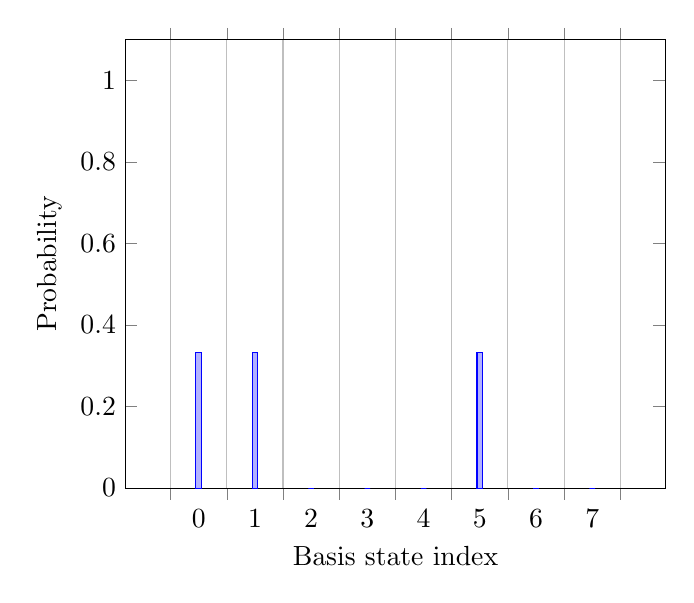
\begin{tikzpicture}
			\begin{axis}[
				ylabel = Probability,
				xlabel = Basis state index,
				ymin = 0,
				ymax = 1.1,
				ybar,
				ybar interval=0.1
			]
			\addplot 
				coordinates {(0,0.333333333333) (1,0.333333333333) (2,0) (3,0) (4,0) (5,0.333333333333) (6,0 ) (7,0) (8,1)};
			\end{axis}
		\end{tikzpicture}
		\caption{Probability distribution for convolution of $\text{T}_a = 11000100$ and $\overline{\text{P}}_a = 10000000$.}
		\label{fig:convolution-a}
	\end{figure}
	\begin{figure}
			\centering
			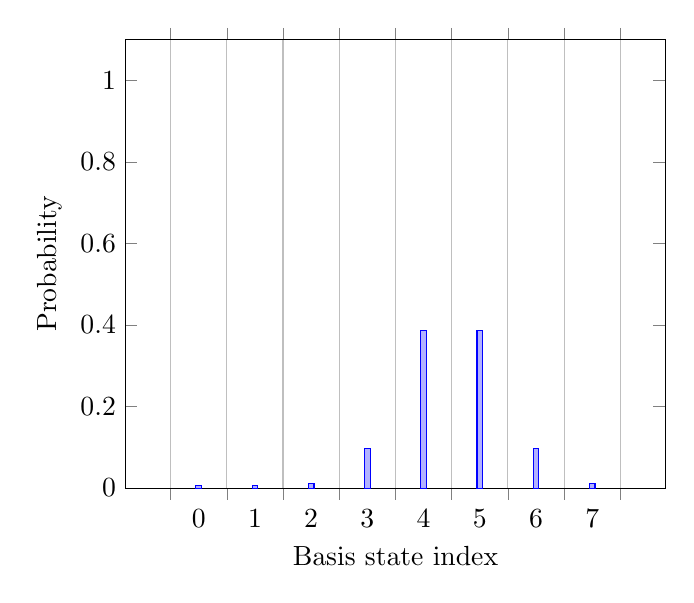
\begin{tikzpicture}
				\begin{axis}[
					ylabel = Probability,
					xlabel = Basis state index,
					ymin = 0,
					ymax = 1.1,
					ybar,
					ybar interval=0.1
				]
				\addplot 
					coordinates {(0,0.0055890168383) (1,0.0055890168383) (2,0.0107053460004) (3,0.0970357555674) (4,0.386669881594) (5,0.386669881594) (6,0.0970357555674 ) (7,0.0107053460004) (8,0)};
				\end{axis}
			\end{tikzpicture}
			\caption{Probability distribution for convolution of $\text{T}_b = 00111000$ and $\overline{\text{P}}_b = 01100000$.}
			\label{fig:convolution-b}
		\end{figure}
	
In Table~\ref{tab:convolution-a}, $0.333333333333 = \frac{1}{3}$ and $3.85185988877e^{-34} \approx 0$. Then, the only possible resulting values of a measurement operation on the current state of register $\alpha$ will be the indices 0, 1 and 5. These values correspond to the substrings $\text{T}_a[0, 0] = 1$, $\text{T}_a[0,1] = 11$ and $\text{T}_a[3,5] = 001$. In Table~\ref{tab:convolution-b}, the order of the indices in T according to probability of occurrence are as follows: 4 and 5, 3 and 6, 7 and 2, and lastly 1 and 0.
\end{example}

\begin{lemma}\label{lem:quantum-convolution-approximate}
	Algorithm~\ref{alg:qca} computes an approximation of the convolution of two binary sequences $\binseq{x}{\sigma}, \binseq{y}{\sigma}$ up to a global multiplicative factor
	\[
		\frac{1}{\sqrt{t_{\mathrm{x}}t_{\mathrm{y}}}}
	\]
and local multiplicative factor
	\[
		\frac{1}{\left\vert \frac{1}{\sqrt{L}}\frac{1}{\sqrt{\binseq{t}{x}}} \sum_{i=0}^{L-1} w^{ij}\binseq{x}{\sigma}[i] \right\vert}
	\]
where $t_{\mathrm{x}}, t_{\mathrm{y}}$ corresponds to the number of 1s in $\binseq{x}{\sigma}, \binseq{y}{\sigma}$, respectively, and $w^{ij}=e^{2\pi i \frac{ij}{L} }$ for all $j=0,\ldots,L-1$.
\end{lemma}

\begin{proof}
Operators $F$ and $F_{\mathrm{Q}}$ have the same unitary matrix representation given by
	\[
		F(i,j) = F_{\mathrm{Q}}(i,j) = \frac{1}{\sqrt{L}} w^{ij}
	\]
	for all $i,j=0,\ldots,L-1$. Same is true with their inverses,
	\[
		F^{-1}(i,j) = F_{\mathrm{Q}}(i,j) = \frac{1}{\sqrt{L}} w^{-ij}
	\]
for all $i=0,\ldots,L-1$. In the quantum setting, $\binseq{x}{\sigma}, \binseq{y}{\sigma}$ have a multiplicative factor of $\frac{1}{\sqrt{t_{\mathrm{x}}}}, \frac{1}{\sqrt{t_{\mathrm{y}}}}$, respectively. Step 1 of Algorithm~\ref{alg:qca} will transform $\binseq{x}{\sigma},\binseq{y}{\sigma}$ into sequences given by
\begin{align*}
	\langle j \myket{\binseq{X}{\sigma}} &= \langle j \vert \fq{\myket{\binseq{x}{\sigma}}}\\
	                                                        &= \frac{1}{\sqrt{L}} \frac{1}{\sqrt{t_{\mathrm{x}}}} \sum_{i=0}^{L-1} w^{ij} \binseq{x}{\sigma}[i]\\
	\langle j \myket{\binseq{Y}{\sigma}} &= \langle j \vert \fq{\myket{\binseq{y}{\sigma}}}\\
	                                                        &= \frac{1}{\sqrt{L}} \frac{1}{\sqrt{t_{\mathrm{y}}}} \sum_{i=0}^{L-1} w^{ij} \binseq{y}{\sigma}[i].
\end{align*}
Step 2 of Algorithm~\ref{alg:qca} corresponds to the point-wise multiplication step of the classical convolution algorithm and will transform $\myket{\binseq{X}{\sigma}}, \myket{\binseq{Y}{\sigma}}$ into the sequence given by
\begin{align*}
	\langle j \vert \V{X}{\binseq{Y}{\sigma}} = \frac{1}{L} \frac{1}{\sqrt{\binseq{t}{x}\binseq{t}{y}}} \left(\frac{\sum_{i=0}^{L-1} w^{ij} \binseq{x}{\sigma}[i]}{\left\vert \frac{1}{\sqrt{L}}\frac{1}{\sqrt{\binseq{t}{x}}} \sum_{i=0}^{L-1} w^{ij} \binseq{x}{\sigma}[i] \right\vert}\right)\left( \sum_{i=0}^{L-1} w^{ij} \binseq{y}{\sigma}[i] \right)
\end{align*}
for all $j=0,\ldots,L-1$. At this point, the quantum convolution algorithm already differs from the classical convolution algorithm by a global multiplicative factor of 
\[
	\frac{1}{\sqrt{\binseq{t}{x}\binseq{t}{y}}}
\] 
and a local multiplicative factor of
\[
	\frac{1}{\left\vert \frac{1}{\sqrt{L}} \frac{1}{\sqrt{\binseq{t}{x}}} \sum_{i=0}^{L-1} w^{ij} \binseq{x}{\sigma}[i] \right\vert}
\]
for all $j=0,\ldots,L-1$.
\end{proof}
%We constructively go through each step of the quantum convolution algorithm and compare the resulting states to that of the classical convolution algorithm. Let the binary indicator sequences $S_1= \alpha_0,\ldots,\alpha_{2^n-1}$ and $S_2=\beta_0,\ldots,\beta_{2^n-1}$ be the input sequences to the Classical convolution algorithm with respect to the symbol $\sigma \in \Sigma$. Let the quantum states
%	\[
%		\vert \alpha_{\sigma} \rangle_0 = \sqrt{\frac{1}{c_\sigma^\text{T}}} \sum_{i=0}^{2^n-1} \alpha_i \vert i \rangle
%	\] 
%	and
%	\[
%		\vert \beta_{\sigma} \rangle_0 = \sqrt{\frac{1}{c_\sigma^{\overline{\text{P}}}}} \sum_{i=0}^{2^n-1} \beta_i \vert i \rangle
%	\] 
%	be the quantum state encoding of the binary indicator sequences $S_1$ and $S_2$. These states will serve as input into the quantum convolution algorithm. $c_\sigma^\text{T}$ and $c_\sigma^{\overline{\text{P}}}$ corresponds to the number of occurrences of symbol $\sigma$ in T and $\overline{\text{P}}$, respectively.
%	
%Step 1 of the classical convolution algorithm results to a vector $X^1$ of values defined such that the \textit{i}-th element of the vector is defined as
%	\begin{align*}
%		X^1_i = \sqrt{\frac{1}{2^n}} \sum_{j=0}^{2^n-1} w^{ij} \alpha_j
%	\end{align*}
%Step 1 of the quantum convolution algorithm results to a quantum superposition state $\vert \alpha_{\sigma} \rangle_1$ defined such that
%	\begin{align*}
%		\langle i \vert \alpha_{\sigma} \rangle_1 = \sqrt{\frac{1}{2^n}} \sqrt{\frac{1}{c_\sigma^\text{T}}} \sum_{j=0}^{2^n-1} w^{ij} \alpha_j
%	\end{align*}
%Step 2 of the classical convolution algorithm will result to a new vector $X^2$ such that its elements are defined as
%	\begin{align*}
%		X^2_i = \sqrt{\frac{1}{2^n}} \sum_{j=0}^{2^n-1} w^{ij} \beta_j
%	\end{align*}
%Step 2 of quantum convolution algorithm will result to a quantum superposition state $\vert \beta_{\sigma} \rangle_1$ defined such that
%	\begin{align*}
%		\langle i \vert \beta_{\sigma} \rangle_1 = \sqrt{\frac{1}{2^n}} \sqrt{\frac{1}{c_\sigma^{\overline{\text{P}}}}} \sum_{j=0}^{2^n-1} w^{ij} \beta_j
%	\end{align*}
%Step 3 of the classical convolution algorithm will result to a vector $Y$ with values defined as
%	\begin{align*}
%		Y_i = \frac{1}{2^n}  \left( \sum_{j=0}^{2^n-1} w^{ij} \alpha_j \right) \left( \sum_{j=0}^{2^n-1} w^{ij} \beta_j \right)
%	\end{align*}
%Step 3 of the quantum convolution algorithm will result to a quantum superposition state $\vert \alpha_{\sigma} \rangle_2$ defined such that
%	\begin{align*}
%		\langle i \vert \alpha_{\sigma} \rangle_2 = \frac{1}{2^n} \sqrt{\frac{1}{c_\sigma^{\overline{\text{P}}}}} \sqrt{\frac{1}{c_\sigma^\text{T}}} \frac{ \left( \sum_{j=0}^{2^n-1} w^{ij} \alpha_j \right) \left( \sum_{j=0}^{2^n-1} w^{ij} \beta_j \right) }{ \bigg\vert \sqrt{\frac{1}{c_\sigma^{\overline{\text{P}}}}} \sum_{j=0}^{2^n-1} w^{ij} \alpha_j \bigg\vert }
%	\end{align*}
%The complex amplitudes in the resulting state $\vert \alpha_{\sigma} \rangle_2$ differs from the elements of vector $Y$ by a multiplicative factor
%	\begin{align*}
%		\sqrt{\frac{1}{c_\sigma^{\overline{\text{P}}}}} \sqrt{\frac{1}{c_\sigma^\text{T}}} \frac{1}{\bigg\vert \sqrt{\frac{1}{c_\sigma^{\overline{\text{P}}}}} \sum_{j=0}^{2^n-1} w^{ij} \alpha_j \bigg\vert}
%	\end{align*}
%Step 4 of the classical convolution algorithm will result to a vector $Z$ of elements defined such that
%	\begin{align}
%		\label{eqn:classical-convolution-algorthim-step-4}
%		Z_k &= \frac{1}{2^n} \sqrt{\frac{1}{2^n}} \sum_{l=0}^{2^n-1} w^{-kl} \sum_{i=0}^{2^n-1} \left( \sum_{j=0}^{2^n-1} w^{ij} \alpha_j \right) \left( \sum_{j=0}^{2^n-1} w^{ij} \beta_j \right)\\
%		&= \frac{1}{2^n} \sqrt{\frac{1}{2^n}} \sum_{j=0}^{2^n-1} \alpha_j \beta_{i-j}
%	\end{align}
%for $k = 0, \ldots, N+M-1$.	 Step 5 of the classical convolution algorithm will result to a vector $C$ with elements defined as
%	\begin{align}
%		C_i = \sum_{j=0}^{2^n-1} \alpha_j \beta_{i-j}
%	\end{align}
%Vector $C$ is the convolution of sequences $S_1$ and $S_2$. Step 4 of the quantum convolution algorithm transforms the state of the quantum register from state $\vert \alpha_\sigma \rangle_2$ into the quantum superposition state $\vert \alpha_{\sigma} \rangle_3$ defined such that
%	\begin{align}
%		\label{eqn:quantum-convolution-algorthim-step-4}
%		\langle k \vert \alpha_{\sigma} \rangle_3 = \frac{1}{2^n} \sqrt{\frac{1}{2^n}} \sqrt{\frac{1}{c_\sigma^{\overline{\text{P}}}}} \sqrt{\frac{1}{c_\sigma^\text{T}}} \sum_{l=0}^{2^n-1} w^{-kl} \Bigg( \sum_{i=0}^{2^n-1} \frac{ \left( \sum_{j=0}^{2^n-1} w^{ij} \alpha_j \right) \left( \sum_{j=0}^{2^n-1} w^{ij} \beta_j \right) }{ \bigg\vert \sqrt{\frac{1}{2^n}} \sqrt{\frac{1}{c_\sigma^{\overline{\text{P}}}}} \sum_{j=0}^{2^n-1} w^{ij} \alpha_j \bigg\vert } \Bigg)
%	\end{align}
%Based from Equations~\ref{eqn:classical-convolution-algorthim-step-4} and \ref{eqn:quantum-convolution-algorthim-step-4}, the quantum convolution algorithm approximates the classical convolution of two binary sequences of up to an overall normalizing multiplicative factor
%	\begin{align*}
%		\sqrt{\frac{1}{c_{\sigma}^{\overline{\text{P}}}}}\sqrt{\frac{1}{c_{\sigma}^{\text{T}}}}
%	\end{align*}
%and a local normalizing factor
%	\begin{align*}
%		\frac{1}{\bigg\vert \sqrt{\frac{1}{2^n}} \sqrt{\frac{1}{c_\sigma^{\overline{\text{P}}}}} \sum_{j=0}^{2^n-1} w^{ij} \alpha_j \bigg\vert}
%	\end{align*}
%These multiplicative factors are necessary to qualify the computation of the quantum convolution algorithm as a valid quantum computation.
%\end{proof}

%AQC makes use of a different encoding scheme as compared to what is used in the classical setting as presented in Section~\ref{sec:cc-encoding} due to some limitations resulting from requirements for a quantum system. Instead, it makes use of binary indicator sequences to encode T and P with respect to each symbol in $\Sigma$ (Section~\ref{subsec:binary-indicator-vectors}). Also, since the input to the problem is in classical encoding there is an additional quantum encoding step prior execution of AQC (Section~\ref{subsec:aqc-encoding}). This is of course common to quantum algorithms since input data to these algorithms are necessarily encoded into quantum memory registers prior to actual computation. 

%========== Consider adding to Appendix
%In the classical setting we encode the input strings T and P into sequences of 1s and -1s by using some functions $f(\cdot)$ and $g(\cdot)$. 
%
%\begin{example}
%\label{classical-encoding-example}
%	Given strings T = aabbba and P = bba and functions $f(\cdot)$ and $g(\cdot)$ defined such that
%	\begin{align*}
%		f(i) =
%		\begin{cases}
%			-1 & \text{ if } T[i] = a\\
%			1 & \text{ if } T[i] = b\\
%		\end{cases}
%		\ \ \text{ and }\ \
%		g(i) =
%		\begin{cases}
%			-1 & \text{ if } P[i] = a\\
%			1 & \text{ if } P[i] = b\\
%		\end{cases}
%	\end{align*}
%	the encoding of T with respect to $f(\cdot)$ is 
%	\begin{align*}
%		T^f &= f(0),f(1),f(2),f(3),f(4),f(5)\\
%				&= -1,-1,1,1,1,-1
%	\end{align*}
%	and the encoding of P with respect to $g(\cdot)$ is
%	\begin{align*}
%		P^g &= g(0),g(1),g(2)\\
%				&= 1,1,-1\ .
%	\end{align*}
%\end{example}
%
%Providing $T^f$ and $\overline{P^g}$ into the classical convolution algorithm and performing some final steps on the resulting values gives us a sequence of values corresponding to the number of matches of each candidate subsequence of T when compared against P. 
%
%\begin{example}
%	Given the encoding of T and $\overline{P}$ in Example~\ref{classical-encoding-example} and providing them as input to classical convolution algorithm, the resulting sequence of values will be the corresponding number of matches less number of mismatches for each valid subsequence of T,
%	\begin{align*}
%		Z &= 1 - 0, 1 - 1, 0 - 3, 1 - 2, 2 - 1, 3 - 0, 1 - 1, 0 - 0\\
%			&= 1, 0, -3, -1, 1, 3, 0, 0
%	\end{align*}
%	Adding $M=3$ to each value and dividing each resulting value with 2 will result to a sequence of values corresponding to the number of matches for each subsequence of T,
%	\begin{align*}
%		C &= \frac{1+3}{2},\frac{0+3}{2}, \frac{-3+3}{2}, \frac{-1+3}{2}, \frac{1+3}{2}, \frac{3+3}{2}, \frac{0+3}{2}, \frac{0+3}{2}\\
%			&= 2, 1\frac{1}{2}, 0, 1, 2, 3, 1\frac{1}{2}, 1\frac{1}{2}
%	\end{align*}
%\end{example}
%
%In the quantum setting we also need to encode first the input strings into a sequence of representative values so we can provide them as input into the AQC algorithm. One way of encoding data into quantum systems is to encode it into the amplitude of the quantum states of the system. The quantum operators which will be used in the AQC algorithm will be operating on the complex amplitudes and so encoding data into the amplitudes of quantum states instead of the quantum states will be more appropriate. Intuitively, we may just follow the encoding scheme we used in the classical setting for the quantum encoding which is to map the value $-1$ to the symbol '\textit{a}' and $1$ to the symbol '\textit{b}' via functions $f(\cdot)$ and $g(\cdot)$.
%\begin{example}
%	Given the encoding of T and P into $T^f$ and $P^g$ in Example \ref{classical-encoding-example} and adopting its encoding scheme for the quantum encoding of T and P we will have the following quantum states
%\begin{align*}
%	\vert \alpha \rangle = -\sqrt{\frac{1}{6}}\vert 000 \rangle -\sqrt{\frac{1}{6}}\vert 001 \rangle + \sqrt{\frac{1}{6}}\vert 010 \rangle + \sqrt{\frac{1}{6}}\vert 011 \rangle + \sqrt{\frac{1}{6}}\vert 100 \rangle - \sqrt{\frac{1}{6}}\vert 101 \rangle
%\end{align*}
%corresponding to $T^f$ and
%\begin{align*}
%	\vert \beta \rangle = -\sqrt{\frac{1}{3}} \vert 000 \rangle + \sqrt{\frac{1}{3}} \vert 001 \rangle + \sqrt{\frac{1}{3}} \vert 010 \rangle
%\end{align*}
%corresponding to $\overline{P^g}$.	
%\end{example}
%This encoding scheme though will not be of practical use for the AQC algorithm as detailed in Appendix \ref{app:encoding}. Instead, we use a different encoding scheme which is also often used in the classical setting.
%
%We use a new set of functions $F(\cdot)$ and $G(\cdot)$ for the quantum encoding of T and P defined such that
%%\begin{align*}
%%	F(i) = 
%%	\begin{cases}
%%		
%%	\end{cases}
%%\end{align*}
%
%\begin{example}
%	
%\end{example}
%
%Since we are only considering binary alphabets
%
%In the classical setting we encode each symbol of T and P as the state of a set of distinct bits. The encoding of T and P are then sequences of states of distinct sets of bits.  

%================================

%%%%%%%%%%%%%%%%%%%%%%%%% Correctness of Result %%%%%%%%%%%%%%%%%%%%%%%%%
%\note{Consider removing this section. Proof of correctness is by construction.}
%\section{Correctness of Result}
%\label{sec:correctness}
%The classical algorithm for approximate string matching which makes use of the convolution method provides as output a classical register of size $N+M-1$ with data at each index $i \in \{~0~,~\ldots~,~N~+~M~-~2~\}$ as
%
%\[
%	M - d\left(P, T[i, i+M-1] \right)
%\]
%which is the number of matches between P and the substring $\text{T}[i, \ldots, i+M-1]$. This algorithm provides all the solution in a single iteration. On the other hand, since QASM makes use of quantum memory registers for data storage, only a single index $i \in \{0, \ldots, N~+~M~-~2~\}$ will result from a single execution of the quantum algorithm and thus the need for several iterations.
%
%For the execution of sub-routine AQC for each symbol $\sigma \in \Sigma$ in Step~\ref{alg:qasm:step:aqc} of Algorithm~\ref{alg:qasm} the expected number of iterations in order for a substring $T_\sigma[i,i+M-1]$ of the binary indicator sequence $T_\sigma$ to be included into set $C_\alpha$ is
%\begin{align}
%	\frac{1}{\vert \langle i \vert \alpha_{b_3} \rangle \vert^2}
%\end{align}
%This shows that substrings of the binary indicator sequences $T_\sigma$ with greater number of matches compared to P will require less expected number of iterations to come out as result of measurement in Step~\ref{alg:qasm:step:M} of Algorithm~\ref{alg:qasm} and then to be included into set $C_\sigma$.

\subsection{Verification of classical result}\label{subsec:verification-classical-result}
For each iteration \textit{j} of Algorithm~\ref{alg:qca} we measure each quantum superposition state $\myket{\binseq{z}{\sigma_i}}$ to get a classical value $z_{\sigma_{i}}^j \in \{0,\ldots,N+M-1\}$, for $i=\{0,\ldots,L-1\}$. We record each resulting classical value $z_{\sigma_{i}}^j$ in a table $A_{\mathrm{T},\mathrm{P}}$ as described in Table~\ref{tab:A_matrix}. Recall function $g:\Sigma \rightarrow \{0,\ldots,M-1\}$ defined in Section~\ref{sec:application-to-approximate-string-matching}. Table $A_{\mathrm{T},\mathrm{P}}$ is defined such that
\[
	A_{\mathrm{T},\mathrm{P}}(i,j) = z_{\sigma_{i}}^j - g(\sigma_i)
\]
for all $i=1,\ldots,\vert \Sigma \vert$ and $j=1,\ldots,K$. We record the unique values in $A_{\mathrm{T},\mathrm{P}}$ where $M-1 \leq A_{\mathrm{T},\mathrm{P}}(i,j) \leq N-M+1$ in an ordered set $B_{\mathrm{T},\mathrm{P}}$, from highest to lowest number of occurrence in $A_{\mathrm{T},\mathrm{P}}$.

Each element in $B_{\mathrm{T},\mathrm{P}}$ can be verified classically by checking if
\[
	H\left( \mathrm{P}, \mathrm{T}[B_{\mathrm{T},\mathrm{P}}(i)],\ldots,\mathrm{T}[B_{\mathrm{T},\mathrm{P}}(i) + M - 1] \right) \leq d
\]
for all $i=1,\ldots,K$. Classical verification can be performed in $\Om\left( M \right)$ time steps.

%%%%%%%%%%%%%%%%%%%%%%%%% QASM algorithm %%%%%%%%%%%%%%%%%%%%%%%%%
\section{Quantum algorithm 2}\label{sec:quantum-algorithm-2}
In Algorithm~\ref{alg:convolution-based-quantum-algorithm} we define an algorithm which makes use of the ESQUID algorithm and quantum convolution algorithm for solving the approximate string matching problem. We let $Sol = \{ \}$ initially.

%Given the sub-routines presented in the previous sections, Quantum algorithm 2 is defined in Algorithm~\ref{alg:quantum-algorithm-2}.
\begin{algorithm}
	\caption{Convolution-based quantum algorithm for approximate string matching}
	\label{alg:convolution-based-quantum-algorithm}
	\begin{algorithmic}[1]
		\REQUIRE{text $\mathrm{T} \in \Sigma^N$, pattern $\mathrm{P} \in \Sigma^M$, Hamming distance constraint \textit{d}}
		\ENSURE{set of indices \textit{i} such that $H(\mathrm{P},\mathrm{T}[i],\ldots,\mathrm{T}[i+M-1]) \leq d$}
		\FOR{ j=1,\ldots,K}
			\FORALL {$\sigma_i \in \Sigma$}
				\STATE $\myket{\binseq{T}{\sigma_i}} = \mathrm{ESQUID}(\binseq{T}{\sigma_i})$
				\STATE $\myket{\binseq{P}{\sigma_i}} = \mathrm{ESQUID}(\binseq{P}{\sigma_i})$
				\STATE $\myket{\binseq{z}{\sigma_i}} = \mathrm{QCON}(\myket{\binseq{T}{\sigma_i}},\myket{\binseq{P}{\sigma_i}})$
				\STATE $\mathrm{z}^j_{\sigma_i} = \mathrm{M}\left( \myket{z_{\sigma_i}} \right)$
				\STATE $A_{\mathrm{T},\mathrm{P}}(i,j) = g(\sigma_i) - \mathrm{z}^j_{\sigma_i}$
			\ENDFOR
		\ENDFOR
		\STATE Construct $B_{\mathrm{T},\mathrm{P}}$ from $A_{\mathrm{T},\mathrm{P}}$.
		\FORALL {$i \in B_{\mathrm{T},\mathrm{P}}$}
			\IF {$H\left( \mathrm{P}, \mathrm{T}[i],\ldots,T[i + M - 1] \right) \leq d $}
				\STATE $Sol \cup \{i\}$
			\ENDIF
		\ENDFOR
		\RETURN \textit{Sol}
		
%		\STATE Encode T and P into binary indicator sequences $\text{T}_a$, $\overline{\text{P}}_a$, $\text{T}_b$ and $\overline{\text{P}}_b$ using sub-routine CEncode(T,P).
%		\FOR{$i=0$ to $j$}
%			\FOR{\textbf{each} $\sigma \in \Sigma=\{a,b\}$ }
%				\STATE Encode $\text{T}_{\sigma}$ and $\overline{\text{P}}_{\sigma}$ into the state of quantum registers QRegT and QRegP respectively using sub-routine ESQUID($\vert \psi_{map} \rangle$). \label{alg:qasm:qencode}
%				\STATE Perform convolution on the state of QRegT and QRegP using sub-routine AQC($\vert \alpha_\sigma \rangle$,~$\vert \beta_\sigma \rangle$). \label{alg:qasm:step:aqc}
%				\STATE Measure the state of QRegT. \label{alg:qasm:step:M}
%				\STATE Add resulting classical value \textit{k} less $\left(M-1\right)$ to set $C_{\sigma}$.
%			\ENDFOR
%		\ENDFOR
%		\STATE Get the union of sets $C_a$ and $C_b$, $C=C_a \cup C_b$.
%		\FOR{\textbf{each} $i \in C$}
%			\IF{ $d(\text{T}[i,i+M-1],\text{P}) \leq D$ }
%				\STATE Add \textit{i} to $C^\prime$
%			\ENDIF
%		\ENDFOR
%		\STATE Return $C^\prime$
	\end{algorithmic}
\end{algorithm}

\begin{theorem}
There exists a quantum algorithm which outputs \textit{k} starting indices of approximate copies $\mathrm{T}[i],\ldots,\mathrm{T}[i+M-1]$ of P in T in time complexity
\[
	\Om\left( K\left(\log_2^2 L + q\log_2 L\right)\right)
\]
with each index having the probability
\[
   \prod_{\sigma \in \Sigma} \left\vert \frac{1}{L\sqrt{L}}\frac{1}{\sqrt{t^{\mathrm{T}}_{\sigma}t^{\mathrm{P}}_{\sigma}}}  \left[ \sum_{j=0}^{L-1} w^{-jl} \left[ \left(\frac{\sum_{i=0}^{L-1} w^{ij}\cdot\mathrm{T}_{\sigma}[i]}{\left\vert \frac{1}{\sqrt{L}}\frac{1}{\sqrt{t^{\mathrm{T}}_{\sigma}}} \sum_{i=0}^{L-1} w^{ij}\cdot\mathrm{T}_{\sigma}[i] \right\vert}\right)\left( \sum_{i=0}^{L-1} w^{ij}\cdot\mathrm{P}_{\sigma}[i]\right)  \right] \right] \right\vert^2
\]
where $L=N+M-, q \ll L, k \ll K, w^{\pm jl}=e^{\pm 2\pi i j\frac{l}{L}}$, and $t^{\mathrm{T}}_{\sigma}, t^{\mathrm{P}}_{\sigma}$ is the number of occurrence of symbol $\sigma$ in the binary indicator sequence $\mathrm{T}_{\sigma}$ and $\mathrm{P}_{\sigma}$ respectively.
\end{theorem}
\begin{proof}
By Lemma~\ref{lem:quantum-convolution-time-complexity}, the computed total time complexity of computing for the convolution of two binary indicator sequences $\mathrm{T}_{\sigma}$ and $\mathrm{P}_{\sigma}$, $\sigma \in \Sigma$ is 
\[
	\Om\left( \log_2^2 L + q\log_2 L \right).
\]
In Section~\ref{sec:time-space-complexity}, the number of iterations of the quantum convolution algorithm is bounded as
\[
	K \in \Om\left(\frac{L\log_2 L + L}{\log_2^2 L + q\log_2 L}\right)
\]
By Lemma~\ref{lem:quantum-convolution-approximate}, each state $\vert l \rangle$ in the quantum convolution of the pair of binary indicator sequences $\mathrm{T}_{\sigma}, \mathrm{P}_{\sigma}$ has amplitude
\[
	\frac{1}{L\sqrt{L}}\frac{1}{\sqrt{t^{\mathrm{T}}_{\sigma}t^{\mathrm{P}}_{\sigma}}}  \left[ \sum_{j=0}^{L-1} w^{-jl} \left[ \left(\frac{\sum_{i=0}^{L-1} w^{ij}\cdot\mathrm{T}_{\sigma}[i]}{\left\vert \frac{1}{\sqrt{L}}\frac{1}{\sqrt{t^{\mathrm{T}}_{\sigma}}} \sum_{i=0}^{L-1} w^{ij}\cdot\mathrm{T}_{\sigma}[i] \right\vert}\right)\left( \sum_{i=0}^{L-1} w^{ij}\cdot\mathrm{P}_{\sigma}[i]\right)  \right] \right].
\]
The probability of getting an index \textit{l} as starting index of an approximate copy of P in T is then the product of the probabilities of getting \textit{k} as classical result of measuring the quantum convolution of binary indicator sequences $\mathrm{T}_{\sigma}$ and $\mathrm{P}_{\sigma}$ for all $\sigma \in \Sigma$, which is given by
\[
   \prod_{\sigma \in \Sigma} \left\vert \frac{1}{L\sqrt{L}}\frac{1}{\sqrt{t^{\mathrm{T}}_{\sigma}t^{\mathrm{P}}_{\sigma}}}  \left[ \sum_{j=0}^{L-1} w^{-jl} \left[ \left(\frac{\sum_{i=0}^{L-1} w^{ij}\cdot\mathrm{T}_{\sigma}[i]}{\left\vert \frac{1}{\sqrt{L}}\frac{1}{\sqrt{t^{\mathrm{T}}_{\sigma}}} \sum_{i=0}^{L-1} w^{ij}\cdot\mathrm{T}_{\sigma}[i] \right\vert}\right)\left( \sum_{i=0}^{L-1} w^{ij}\cdot\mathrm{P}_{\sigma}[i]\right)  \right] \right] \right\vert^2
\]
\end{proof}

%Since any quantum computation only returns a single classical value at the end of its computation, the quantum sub-routines ESQUID and AQC needs to be invoked multiple times. Also, since we encode the classical input T and the reverse of P into binary indicator sequences, we need to execute ESQUID and AQC for each encoding of T and P with respect to each symbol $\sigma \in \Sigma$. 

%ESQUID and AQC sub-routines can be performed in parallel for each symbol $\sigma$ though. We need to allocate $2\vert \Sigma \vert$ quantum memory registers to accommodate the input data.
%\begin{example}
%\label{exa:qasm}
%	Given input strings $\text{T}= aabbba$ and $\text{P}= bba$ and Hamming distance constraint $\text{D}=2$ we invoke QASM as $\text{QASM}(aabbba, bba, 2)$. CEncode(T,P) will encode T and P with respect to symbols '\textit{a}' and '\textit{b}' as $\text{T}_a = 110001$, $\text{T}_b = 001110$, $\overline{\text{P}}_a = 100$ and $\overline{\text{P}}_b = 011$. ESQUID will encode $\text{T}_a$, $\overline{\text{P}}_a$, $\text{T}_b$ and $\overline{\text{P}}_b$ into quantum superposition states
%	\begin{align*}
%		\vert \alpha_a \rangle &= \sqrt{\frac{1}{3}}\vert 000 \rangle + \sqrt{\frac{1}{3}}\vert 001 \rangle + \sqrt{\frac{1}{3}}\vert 101 \rangle\ ,\\
%		\vert \beta_a \rangle &= \vert 000 \rangle\ ,\\
%		\vert \alpha_b \rangle &= \sqrt{\frac{1}{3}}\vert 010 \rangle + \sqrt{\frac{1}{3}}\vert 011 \rangle + \sqrt{\frac{1}{3}}\vert 100 \rangle\ ,\\
%		\vert \beta_b \rangle &= \sqrt{\frac{1}{2}}\vert 000 \rangle + \sqrt{\frac{1}{2}}\vert 001 \rangle
%	\end{align*}
%	respectively. AQC will then be invoked both for symbol '\textit{a}' and '\textit{b}'. Invoking $\text{AQC}(\vert \alpha_a \rangle, \vert \beta_a \rangle)$ will result to the quantum superposition state
%	\begin{align*}
%		\vert \tau_a \rangle &\approx K_a \left( 1\cdot \vert 000 \rangle + 1\cdot \vert 001 \rangle + 0\cdot \vert 010 \rangle + 0\cdot \vert 011 \rangle + 0\cdot \vert 100 \rangle + 1\cdot \vert 101 \rangle + 0\cdot \vert 110 \rangle + 0\cdot \vert 111 \rangle \right)\\
%		&\approx K_a\left( \vert 000 \rangle + \vert 001 \rangle + \vert 101 \rangle \right)
%	\end{align*}
%	where
%	\[	
%		K_a = \frac{1}{8}\sqrt{\frac{1}{8}}\sqrt{\frac{1}{3 \cdot 1}}
%	\]
%	and $\text{AQC}(\vert \alpha_b \rangle, \vert \beta_b \rangle)$ to
%	\begin{align*}
%		\vert \tau_b \rangle &\approx K_b\left( 0\cdot\vert 000 \rangle + 0\cdot\vert 001 \rangle + 0\cdot\vert 010 \rangle + 1\cdot\vert 011 \rangle + 2\cdot \vert 100 \rangle + 2\cdot\vert 101 \rangle + 1\cdot\vert 110 \rangle + 0\cdot\vert 111 \rangle \right)\\
%		&\approx K_b\left( \vert 011 \rangle + 2\vert 100 \rangle + 2\vert 101 \rangle + \vert 110 \rangle \right)
%	\end{align*}
%	where
%	\[	
%		K_b = \frac{1}{8}\sqrt{\frac{1}{8}}\sqrt{\frac{1}{3 \cdot 2}}\ .
%	\]
%Classical values $-2, -1$ and $3$, corresponding to indices $000=0, 001=1$ and $101=5$ less $(M-1)$, all have the probability of
%	\begin{align*}
%		&\approx \vert K_a \cdot 1 \vert^2\\
%		&\approx \Bigg\vert \frac{1}{8}\sqrt{\frac{1}{8}}\sqrt{\frac{1}{3 \cdot 1}} \cdot 1 \Bigg\vert^2
%	\end{align*}		
%of being included into the set $C_a$.	Classical values $1$ and $4$, corresponding to indices $011=3$ and $110=6$ less $(M-1)$, have the probability of
%	\begin{align*}
%		&\approx \vert K_b \cdot 1 \vert^2\\
%		&\approx \Bigg\vert \frac{1}{8}\sqrt{\frac{1}{8}}\sqrt{\frac{1}{3 \cdot 2}} \cdot 1 \Bigg\vert^2
%	\end{align*}
%while values $2$ and $3$, corresponding to indices $100=4$ and $101=5$ less $(M-1)$, have probability
%	\begin{align*}
%		&\approx \vert K_b \cdot 2 \vert^2\\
%		&\approx \Bigg\vert \frac{1}{8}\sqrt{\frac{1}{8}}\sqrt{\frac{1}{3 \cdot 2}} \cdot 2 \Bigg\vert^2
%	\end{align*}
%of being included into the set $C_b$. \note{what is optimal value for j?} After some number of iterations \textit{j} we expect to have the set of indices $C^\prime=\{-2,-1,1,2,3,4\}$ where negative values correspond to comparisons in which P is extended to the left of T starting from alignment of $\text{T}[0]$ with $\text{P}[M-1]$. Positive values greater than $N-M+1$ correspond to comparisons in which P is extended to the right of T ending with alignment of $\text{T}[N-1]$ with $\text{P}[0]$. The elements of set $C^\prime$ correspond to the sub-sequences $a$, $aa$, $abb$, $bbb$, $bba$ and $ba$ respectively. When compared with $\text{P}=bba$ these sub-sequences have $2, 2, 2, 1, 0, 2$ number of mismatches, respectively.
%\end{example}

%%%%%%%%%%%%%%%%%%%%%%%%% Time and Space Complexity %%%%%%%%%%%%%%%%%%%%%%%%%
%\section{Time and Space Complexity}
%\label{sec:complexity}
%We compute for the time and space complexity of the sub-routines of Quantum algorithm 2 to compute for its overall complexity. 
%
%The construction of the superposition quantum states representing the strings T and reverse of P, both padded with 0s, using the ESQUID sub-routine will require time complexity $O(\log_2{\left(N+M\right)})$ and space complexity of $O(\log_2{\left(N+M\right)})$. In the AQC algorithm, the \textit{QFT} steps will require $O(\log_2^2{\left(N+M\right)})$ time complexity while the approximation of the dot multiplication step will require $O(N+M)$ time complexity. The linear time complexity for the approximation of the dot multiplication step can be attributed to the resource-intensive implementation of diagonal unitary matrices on quantum circuits using only one- and two-qubit quantum gates. An efficient algorithm for implementing diagonal unitaries without ancilla qubits on quantum circuits can be found in \cite{Welch2014}. The execution of the AQC sub-routine can be done in parallel to compensate for the $\vert \Sigma \vert$ multiplicative factor. The space complexity of the AQC sub-routine is $O(\log_2{\left( N+M \right)})$ since we need to allot quantum registers for both T and the reverse of P. The last loop in Quantum algorithm 2 verifies the found indices in T if they satisfy the input distance requirement and is bounded above by the number of iterations $j$ in the previous loop in Quantum algorithm 2.  
%
%Note that Quantum algorithm 2 is advantageous with regards to computation time steps in comparison to the classical algorithm which uses convolution method if it is the case that 
%\begin{align}
%\label{constraint-on-j}
%	j < \log_2{\left( N+M \right)} \ .
%\end{align}
%where $j$ is bounded above by the number of substrings of T starting at position $i$ and satisfying the distance constraint
%\[
%	d\left(\text{P}, \text{T}[i, i+M-1] \right) \leq D
%\]
%From this we see that the improvement on the time complexity by the Quantum algorithm 2 in comparison to that of Algorithm~\ref{alg:cc} is a reduction from \textit{log}-\textit{linear} to \textit{linear} time steps, with the assumption that the condition \ref{constraint-on-j} is satisfied. 
%\note{Compute for probability of success.}

%\section{Limitations}
%\label{sec:limitations}

%\subsection{Totally no occurrence of P in T}

%%%%%%%%%%%%%%%%%%%%%%%%% Simulation %%%%%%%%%%%%%%%%%%%%%%%%%
%\section{Simulation}

\section{Summary}
In this chapter we presented the concept of convolution and how it applies to the problem of approximate string matching, both in the classical and quantum setting. We presented a convolution-based quantum algorithm for approximate string matching defined in Algorithm~\ref{alg:convolution-based-quantum-algorithm}. It encodes the input strings T and P into binary indicator sequences for all symbols $\sigma \in \Sigma$. These binary indicator sequences are prepared as quantum superposition states which serve as input to the quantum convolution algorithm in Algorithm~\ref{alg:qca}. The algorithm uses ESQUID algorithm \cite{Rosenbaum2009} for generating the quantum superposition state encoding of the binary indicator sequences for T and P. ESQUID algorithm has circuit and time complexity bounded by $\Om\left( \log_2 L \right)$. It uses the same binary indicator sequence registers used all through the algorithm plus two additional ancillary qubits for coding the progress of its state generation process. Its time complexity is in $\Om\left( \log_2 L \right)$.

We outlined the flow of the quantum convolution algorithm in Section~\ref{subsec:qft} and provided details about its sub-routines in Section~\ref{sec:sub-routines}. The quantum Fourier transform has been shown to be exactly implementable in a quantum circuit with circuit depth of $\Om\left( \log_2^2 L + \log_2 L\right)$ in \cite{Shor2004}. Its circuit and time complexity is thus also bounded the same. It works on the same binary indicator sequence registers used in the ESQUID sub-routine and so works on $\log_2 L$ qubits. The same goes for its inverse. The classical point-wise multiplication operation was also implemented using a unitary diagonal matrix $V_\mathrm{X}$ based on the unitary matrix suggested in \cite{Curtis2004}. We introduced a minor revision of the values of $V_{\mathrm{X}}$ to accommodate the case where there exists states $\vert i \rangle$ in superposition state $\vert X \rangle$ which have an amplitude of zero. This is to avoid division by zero in $V_{\mathrm{X}}$. Using the same analysis for operator $W$ in the previous algorithm, we analyzed the the circuit complexity of a quantum circuit for $V_{\mathrm{X}}$ when decomposed using the Clifford+T gate set. The circuit complexity of $V_{\mathrm{X}}$ will be in $\left( \log_2 L \right)$ assuming $q \ll L$ where \textit{q} is the number of distinct phase values along the diagonal matrix of $V_{\mathrm{X}}$ Its time complexity will thus also be bounded the same. Operator $V_{\mathrm{X}}$ will also work on the same binary indicator sequences used in the previous steps.

Given ordered set $B_{\mathrm{T},\mathrm{P}}$, the resulting indices of the quantum convolution algorithm can be verified classically by checking if $H\left( \mathrm{P}, \mathrm{T}[i],\ldots,\mathrm{T}[i+M-1] \right) \leq d$. Parallelizing the verification of the elements of $B_{\mathrm{T},\mathrm{P}}$ by synthesizing a classical circuit of circuit complexity in $\Om\left(KM\log_2 \vert \Sigma \vert \right)$ will give the classical verification step time complexity in $\Om\left( 1 \right)$ only.

The convolution-based quantum algorithm for approximate string matching presented in this chapter has circuit complexity in
\[
	\Om\left( \log_2^2 L + q\log_2 L + KM\log_2 \vert \Sigma \vert \right),
\]
time complexity in
\[
	\Om\left( K\left(\log_2^2 L + q\log_2 L \right) \right),
\]
and space complexity in
\[
	\Om\left(\vert \Sigma \vert\log_2 L + KM\log_2 \vert \Sigma \vert \right).
\]







